
% Puedes cambiar la licencia de este documento con la orden license.
%\license{Todos los derechos reservados.}

% Si usas muchos símbolos conviene que describas lo que significan en un archivo
% aparte (en este caso simbolos.tex).  Si no es el caso puedes comentar esta 
% línea
\listofsymbols{simbolos.tex}

   \portada
\begin{agradecimientos}
\noindent Quiero agradecerle a mi familia, especialmente a mis padres y a mi tío Javier, por haberme brindado la oportunidad de obtener una formación de calidad, ayudándome en todo momento de forma incondicional.

También quiero darle las gracias al tutor de este trabajo, Francisco Moya, por acercar el mundo de la programación a mi vida, y en general, a todos los docentes que me han acompañado en el camino, con especial atención por aquellos que sienten pasión por su trabajo y se la transmiten a sus alumnos.
\end{agradecimientos}	   
\begin{dedicatoria}
Esta obra está dedicada a la memoria de Alan Turing, cuya contribución tecnológica hace posible, entre otras muchas cosas, este trabajo de fin de grado.
\end{dedicatoria}
\begin{resumen}

\noindent Desde hace ya varios años, el auge de empresas tecnológicas asociadas al alquiler vacacional, como Booking\footnote{\url{https://www.booking.com/}} o Airbnb\footnote{\url{https://www.airbnb.es/}}, han propiciado un cambio significativo en la manera que funciona el turismo, dando la oportunidad, tanto a profesionales del sector como a principiantes, de tener visibilidad ante clientes potenciales.

Es un hecho que muchas personas han hecho de este modelo su forma de ganarse la vida, dedicándole a esta tarea su jornada laboral, a tiempo parcial o completo, para gestionar una o varias viviendas de uso turístico. Algunas de las tareas que se desempeñan en estos puestos de trabajo son las siguientes:
\begin{itemize}
\item Actualizar los precios en función de la demanda.
\item Responder las dudas a los clientes.
\item Ofrecer acceso a la vivienda y atender a los usuarios en su llegada.
\item Gestionar los trabajos de limpieza.
\item Prevenir el exceso de ventas para una misma habitación en el mismo día cancelando la disponibilidad de una misma vivienda en distintas plataformas.
\end{itemize}

\noindent En la actualidad existen herramientas que permiten actualizar los precios de forma automática en base a algoritmos que tienen en cuenta la demanda, y también pueden encontrarse algunas que permiten sincronizar los calendarios de las distintas plataformas entre sí, con el fin de facilitar el trabajo de los propietarios de viviendas de uso turístico.

El objeto de este trabajo de fin de grado consiste en gestionar la llegada del cliente a la vivienda de uso turístico, haciendo que las tareas desempeñadas entre el momento en que se realizan las reservas, y el que los clientes acceden a la vivienda, queden completamente automatizados, liberando de esta manera una importante carga de trabajo a los propietarios. El resultado de este trabajo es hacer que el anfitrión de la vivienda de uso turístico pueda tener la garantía de que su negocio se está gestionando de forma automática, y que solo se le avisará en casos particulares, cuando sea estrictamente necesario.

Para llevar a cabo esta tarea se creará un sistema que permita gestionar, de forma automática, por medio de una Raspberry Pi Zero W, la apertura de las puertas de acceso a la vivienda en los momentos que proceda. De igual manera, se integrarán en el sistema todas aquellas tareas que pueden tenerse en cuenta, como las posibles cancelaciones, la organización de los equipos de limpieza o las medidas de seguridad que garantizarán la tranquilidad de aquellos anfitriones que deseen hacer uso de este sistema.

Tanto los usuarios finales, como el administrador, podrán hacer uso de todas estas herramientas a partir de la aplicación de mensajería instantánea "Telegram". La elección de Telegram como aplicación de la plataforma no es casual, si no que responde a unos criterios bien definidos:
\begin{itemize}
\item Telegram es, y siempre ha sido, una aplicación de código abierto, lo cual abre la puerta a posibilidades infinitas de programación, así como la seguridad de saber que el sistema será estable en relación a las políticas de la plataforma. 
\item La inmensa mayoría de la población vive familiarizada con las aplicaciones de mensajería instantánea, por lo que la curva de aprendizaje sería mínima, y ello aceleraría considerablemente la adaptación de los clientes potenciales.
\item Telegram trabaja con un cifrado de 64 bits, de extremo a extremo, en todas sus comunicaciones. Esto facilita considerablemente el trabajo y resulta de gran utilidad a la hora de evitar interceptaciones de información por parte de terceros.
\end{itemize}
\end{resumen}

\begin{abstract}
\noindent For several years now, the rise of technology companies associated with vacation rental, such as Booking\footnote{\url{https://www.booking.com/}} or Airbnb\footnote{\url{https://www.airbnb.es/}}. They have brought about a significant change in the way tourism works, giving professionals, as well as beginners, the opportunity to have visibility before potential clients.

It is a fact that many people have made this model their way of earning a living, dedicating their part-time or full-time workday to this task to manage one or more houses for tourist use. Some of the tasks performed in these jobs are the following:
\begin{itemize}
\item Update prices based on demand.
\item Answer questions to customers.
\item Offer access to housing and attend to users upon arrival.
\item Manage cleaning jobs.
\item Prevent excess sales for the same room on the same day by canceling the availability of the same home on different platforms.
\end{itemize}

\noindent Currently there are tools that allow updating prices automatically based on algorithms that take into account demand, and there are also some that allow synchronizing the calendars of the different platforms with each other, in order to facilitate the work of homeowners for tourist use.

The purpose of this final degree project is to manage the client's arrival at the dwelling for tourist use, making the tasks performed between the time the reservations are made and the clients accessing the dwelling completely automated, thus relieving a significant workload for owners. The result of this work is to ensure that the host of the tourist-use dwelling can have the guarantee that his business is being managed automatically, and that he will only be notified in particular cases, when strictly necessary.

To carry out this task, a system will be created that automatically manages, by means of a Raspberry Pi Zero W, the opening of the access doors to the house at the appropriate times. Likewise, all those tasks that may be taken into account, such as possible cancellations, the organization of cleaning teams, or security measures that will guarantee the tranquility of those hosts who wish to use this system, will be integrated into the system.

Both end users and the administrator will be able to make use of all these tools from the "Telegram" instant messaging application. The choice of Telegram as application of the platform is not accidental, if not that it meets well-defined criteria:
\begin{itemize}
\item Telegram is, and always has been, an open source application, which opens the door to infinite programming possibilities, as well as the security of knowing that the system will be stable in relation to the platform's policies.
\item The vast majority of the population lives familiarized with the applications of instantaneous mail, reason why the learning curve would be minimal, and this would accelerate considerably the adaptation of the potential clients.
\item Telegram works with 64-bit encryption, end-to-end, in all its communications. This considerably facilitates the work and is very useful in avoiding interception of information by third parties.
\end{itemize}
\end{abstract}


\indices

% El cuerpo del documento está en la carpeta tex
% Aquí simplemente se incluyen los archivos correspondientes a cada capítulo.

% No los llames capitulo1, capitulo2, etc. Los números los pondrá LaTeX según
% el orden en que los pongas.  Eso facilitará después su posible reordenación
% o división.

% Esta estructura corresponde al anexo TFG-08b (documento científico-técnico).
% Si ves que tu proyecto concuerda con TFG-08a organiza el documento según
% UNE 157001

\chapter{Introducción} 
\label{ch:introduccion}

\section{Presentación del problema} 
\label{sec:presentacion-del-problema}

\noindent El alquiler de viviendas para uso turístico constituye, sin lugar a dudas, un pilar para el turismo, y por tanto, para la economía en España. El turismo es el sector que más riqueza aporta a la economía española, en términos de producto interior bruto (PIB) y de empleo \cite{hosteltur2020}. No obstante, la integración de sistemas de automatización que tienen por objeto recibir a los clientes en este sector, no alcanza la misma velocidad, ya que en la mayoría de casos se sigue atendiendo a los turistas con el mismo modelo de hace 10 o 15 años.

La mayoría de las viviendas de uso turístico siguen requiriendo una considerable carga de trabajo para sus anfitriones, y lejos de convertirse en un ingreso pasivo, se transforma en un trabajo que requiere atender una por una las nuevas reservas, recibir a los clientes, gestionar al personal de limpieza, responder ante posibles desperfectos, etc. Todo esto hace que muchas personas recurran a alquilar sus viviendas de la forma tradicional, por medio de particulares que harán uso de la misma durante un largo periodo de tiempo, a cambio de un monto inferior al que se recaudaría, en muchas ocasiones, por medio del alquiler turístico.

Un sistema automatizado será capaz, por su naturaleza, de ofrecer servicios más económicos, o de mayor calidad, ya que su costé se verá reducido de forma considerable, y permitirá convertir estos ingresos en pasivos para los propietarios, quienes verán reducida de forma considerable su carga de trabajo, y esto les motivará a formar parte de esta actividad.

Además, esto también jugará a favor de la economía de nuestro país, ya que en las fechas de mayor ocupación podrá tener disponibilidad de un mayor número de plazas para pernoctar, con todos los beneficios que ello implica a nivel económico.

\section{Soluciones propuestas} 
\label{sec:soluciones-propuestas}

\noindent Este trabajo de fin de grado pretende introducir los desarrollos tecnológicos actuales en el mundo de las viviendas de uso turístico, eliminando parte de la carga de trabajo a la que se enfrentan los anfitriones de dichas viviendas. Algunas de las actividades que se pretenden realizar son las siguientes:
\begin{itemize}
\item Atención automatizada del cliente. El anfitrión de la vivienda no tendrá porque saber si alguien ha hecho o no una reserva si no quiere. Este sistema atenderá al cliente en el momento en que realice una reserva, y lo guiará hasta la vivienda, donde se encargará también de ofrecerle acceso.
\item Automatización de las cancelaciones. En caso de que se produzcan cancelaciones, el sistema lo tendrá en cuenta y gestionará debidamente las acciones pertinentes, con el fin de anular el acceso para la persona que ejecuta la cancelación y abrirlo a nuevos clientes potenciales.
\item El proyecto incluirá un panel de administración para el anfitrión, desde el cuál podrá realizar las siguientes tareas:
\begin{itemize}
\item Consultar las reservas existentes. El anfitrión tendrá la posibilidad de consultar todas las reservas que contenga el sistema.
\item Crear nuevas reservas. El anfitrión podrá crear reservas para los días que considere convenientes, desde un panel de gestión implantado en la propia aplicación de Telegram.
\item Anular reservas. De igual manera, el anfitrión tendrá la posibilidad de cancelar aquellas reservas que considere convenientes.
\item Por último, el panel de administración para el anfitrión incluirá la posibilidad de realizar la apertura de las puertas de forma automática.
\end{itemize}
\end{itemize}
Para llevar a efecto la apertura de las puertas se hará uso de una Raspberry Pi Zero W\footnote{\url{https://www.raspberrypi.org/products/raspberry-pi-zero-w/}}. Esta placa, por medio de su programación interna, facilitará la activación del circuito eléctrico que permitirá realizar la apertura de puertas. Además, gestionará la ejecución de todos los programas que se mencionan en el presento proyecto.

En cuanto al uso de Telegram como plataforma de mensajería instantánea, se hará uso de la libreria disponible en python, \emph{PyTelegramBotApi}\footnote{\url{https://github.com/python-telegram-bot/python-telegram-bot}}.

Los programas que se ejecutan trabajan con el envío y la recepción de correos electrónicos, por medio de los cuales realizan la automatización de los procesos. Estos correos electrónicos se enviarán a partir del lenguaje de programación Python con la libreria \emph{smtplib}\footnote{\url{https://github.com/python/cpython/blob/master/Lib/smtplib.py}}.

\section{Organización de la memoria} 
\label{sec:organizacion-memoria}

\noindent La organización de este documento responde a un documento científico-técnico. Se descompone en los siguientes capítulos.

\begin{description}
    \item[\autoref{ch:objetivos}] Enumera y justifica los objetivos del proyecto y establece los límites intrínsecos y extrínsecos de ejecución del TFG.
    \item[\autoref{ch:antecedentes}] Analiza los antecedentes y estado del arte en relación al tema del proyecto.
    \item[\autoref{ch:desarrollo}] Describe todo el proceso de desarrollo del TFG.  Esto incluye la metodología de trabajo empleada y las diferentes etapas o iteraciones que se han llevado a cabo.  No dudes en descomponer el capítulo en varios si aglutina demasiado material.
    \item[\autoref{ch:resultados}] Describe en detalle los resultados obtenidos y las pruebas realizadas. Discute los resultados en relación a los objetivos del proyecto.
    \item[\autoref{ch:conclusiones}] Recopila las principales conclusiones del proyecto y comenta las líneas de trabajo futuro, en caso de que se contemplen.
    \item[\deschyperlink{ch:anexos}{Anexos}] Complementan la información del cuerpo del documento con información técnica útil para reproducir los resultados, pero innecesaria para comprender en su totalidad el TFG realizado.
    \item[\deschyperlink{ch:bibliografia}{Bibliografía}] Recopila las referencias bibliográficas utilizadas en este documento.
\end{description}

\section{Repositorio de información}
\label{sec:repositorio}

\noindent El material generado durante la ejecución de este proyecto está disponible en el repositorio \thegitrepo{}. El material incluye el código \LaTeX{} del presente documento, el código fuente de los programas realizados o modificados, y todos los datos generados en la evaluación de resultados.
\chapter{Motivación y antecedentes}
\label{ch:antecedentes}

\noindent Año tras año, en todos los países occidentales, el modelo de negocio de las plataformas de alquiler vacacional con apartamentos turísticos no deja de crecer \cite{juanjocerezo2018}. La forma en la que se organizan las vacaciones, los viajes de negocios y cualquier actividad que incluya pernoctar, está adaptándose a una nueva forma de economía colaborativa. La repercusión que esto tiene en el mercado es positiva, haciendo que nuestro país vea aumentada su capacidad para acoger turistas, de forma que el producto interior bruto recibe un fuerte impulso.\\
No obstante, este modelo de economía colaborativa no está al acceso de todo el mundo, ya que la atención de los clientes es algo que requiere una importante inversión de tiempo, que no siente resulta compatible con la vida laboral o personal de los potenciales anfitriones.\\
Algunos de los problemas que requieren de la atención y el tiempo de los propietarios de viviendas de uso turístico, han sido automatizados por empresas que, a cambio de tarifas mensuales o anuales, ofrecen diferentes servicios a los clientes:
\begin{itemize}
\item Evitar un exceso de huéspedes para una misma habitación. La mayoría de los propietarios de viviendas de uso turístico, tienen sus anuncios en varias plataformas, como Airbnb, Booking, Homeaway, etc. Esto puede provocar que diferentes personas alquilen la misma propiedad en idénticas fechas, produciendo así un fenómeno de sobre venta, lo cual resulta castigado en la mayoría de los casos por medio de sanciones en dichas plataformas. Para solucionar este problema, las estas plataformas ofrecen ya soluciones\footnote{\url{https://www.airbnb.es/help/article/99/como-sincronizo-mi-calendario-de-airbnb-con-otro-calendario}}, pero además existen múltiples empresas que permiten sincronizar los calendarios, haciendo que al recibir una reserva en una plataforma, las demás queden deshabilitadas para tales fechas, acabando así con este indeseado fenómeno.
\item Responder a los clientes. La mayoría de plataformas de alquiler vacacional, incluyen en su software la posibilidad de ofrecer respuestas automáticas\footnote{\url{https://partner.booking.com/es/ayuda/reservas/}}, de manera que los propietarios de las viviendas no se vean obligados a responder uno por uno a los clientes.
\item Apertura de puertas de forma automática. Existen además empresas que se dedican a implantar sistemas automáticos para la apertura de puertas\footnote{\url{https://raixer.com/funcionamiento/abrir-puertas-automaticamente/}}. Estas aperturas se realizan a través de una petición de usuario, bien por medio de una llamada telefónica, o bien por medio de una aplicación que se puede descargar en Android e iOS.
\item Cálculo automatizado de precios. Optimizar los precios de una vivienda turística puede resultar un auténtico quebradero de cabeza para aquellos que quieran hacerlo de forma acertada. Las grandes cadenas hoteleras funcionan por medio de algoritmos automatizados que actualizan constantemente los precios en función de muchas variables, como la demanda, el tiempo restante, etc. En la actualidad, existen también plataformas que permiten actualizar dichos precios de forma automatizada\footnote{\url{https://hello.pricelabs.co/}}, de manera que el propietario, a cambio de un pago mensual, pueda ahorrarse una cantidad considerable de tiempo y potenciar al máximo la optimización de sus precios.

\end{itemize}

\noindent Como puede observarse, las empresas tecnológicas han apostado por el mercado de los alojamientos turísticos para emprender negocios, optimizando cada vez más esta forma de comercio. Sin embargo, los anfitriones siguen contando con una importante carga de trabajo, que repercute en su capacidad de incorporarse a este modelo de economía colaborativa.

Las motivaciones principales de este trabajo de fin de grado pasan por mejorar, de manera bidireccional, la experiencia de los huéspedes y los anfitriones, así como acercar a estos últimos la posibilidad de poder incluir este modelo de negocio pasivo en su economía personal. A continuación se mencionarán algunas de estas motivaciones de manera más detallada.

\section{Automatización completa del proceso de reserva} 
\label{sec:automatizacion-completa-del-proceso-de-reserva}

\noindent La posibilidad de incluir un sistema automatizado por completo, o uno semi automatizado, puede ser decisiva a la hora de que una persona se decida por el modelo de negocio de las viviendas de uso turístico.

El trabajo y los asuntos personales suelen requerir de una cantidad importante de recursos para las personas, que no siempre disponen del tiempo y la energía suficiente para atender a los turistas, y debido a ello, deciden abandonar este tipo de inversiones.

Este aspecto podría ser distinto, sin embargo, si por medio de un sistema automatizado, el anfitrión pudiera tener la tranquilidad de saber que su negocio se está gestionando solo, ya que de esta manera si podría plantearse esta inversión sabiendo que no le requerirá invertir tiempo de forma diaria. Un sistema que atienda de principio a fin al cliente, organizando cada reserva y ofreciendo el acceso a la vivienda, podría dar una solución definitiva a este problema y, de esta manera, abrir este terreno a multitud de potenciales anfitriones.

\section{Uso de aplicaciones de mensajería instantánea} 
\label{sec:uso-de-aplicaciones-de-mensajeria-instantanea}

\noindent En la actualidad, recientes estudios \cite{itreseller2019} afirman que el 85 por ciento de los españoles utiliza aplicaciones de mensajería instantánea. Para cualquier modelo de negocio, incluir una nueva tecnología en la que la curva de aprendizaje sea mínima, tendrá siempre un impacto positivo en la supervivencia de su fase inicial. En este caso, hacer que todo este sistema se automatice por medio de aplicaciones de mensajería instantánea hará que se facilite su uso a la inmensa mayoría de la población.

Además, según un estudio \cite{samuelfernandez2019} realizado por Telefónica, se ha demostrado que el 95,1\% de los españoles prefiere enviar un mensaje a realizar una llamada, por lo que se demuestra, una vez más, la validez de este método como forma de gestión de estos negocios al alza.

\section{Estado del arte}

\noindent El internet de las cosas, según Wikipedia\footnote{\url{https://es.wikipedia.org/wiki/Internet_de_las_cosas}} se define como la interconexión digital de objetos cotidianos por internet.

Su principal objetivo es el de facilitar la vida de las personas, evitando tener que hacer una importante cantidad de trabajos manuales, y en muchas ocasiones, optimizando los resultados obtenidos respecto a un humano.

\subsection{Historia del internet de las cosas}

\noindent Como todo avance tecnológico, el internet de las cosas establece su base a partir de otras tecnologías que lo precedieron antes y permitieron su evolución. Es por ello que, a la hora de hacer un análisis histórico, marcar el comienzo es un proceso que implica siempre cierto grado de subjetividad.

En este caso, se establece en 1969 el comienzo del internet de las cosas con el origen del propio internet, año en el que se realizó por primera vez la red operativa ARPANET\cite{tibipuiu2020}. Sin embargo, no fue hasta 1999 cuando, Kevin Asthon, acuñó por primera vez el concepto de internet de las cosas mientras impartía una conferencia en Procter and Gamble.

Tras este suceso, el término empieza a ser más extendido en diversos medios de comunicación, dando lugar durante estos primeros años del siglo XXI al uso de la tecnología RFID\cite{sorayapa2012}, cuyo propósito fundamental es la de transmitir información de los objetos a través de ondas de radio.

El año 2005 supone un año de suma importancia para el internet de las cosas, ya que es el momento en que la agencia de las naciones unidas "International Telecomunications Union (ITU)" reconoce esta materia haciendo público su primer estudio sobre el tema. Adicionalmente, ese año aparece por primera vez Arduino, un tipo de computadora orientada a la detección y control de objetos cotidianos.

Con el fin de hacer una base estable y estandarizada sobre esta materia, en el año 2008 un grupo de empresas importantes se unen para crear IPSO\footnote{\url{https://es.wikipedia.org/wiki/Internet_de_las_cosas}}, con el fin de promover el uso de un protocolo de internet en los objetos inteligentes.

En 2009 se crea la fundación Raspberry Pi\cite{rubenandres2019}, como una asociación caritativa que es regulada por la comisión de caridad de Inglaterra y Galés. Estas computadoras potenciarán activamente a partir de entonces, junto con arduino y otras muchas, la evolución y extensión del internet de las cosas.

En 2010, el número de objetos cotidianos y dispositivos conectados a internet superaba los 12 mil millones\cite{daveevans2011}.

En 2020, se estima que la cantidad de objetos conectados a internet ascenderá a 34 mil millones\cite{martinfernandez2017}.

\subsection{Historia de Raspberry Pi}

\noindent Los primeros diseños de Raspberry pi se efectuaron en el año 2006. Sin embargo, no fue hasta 2009 cuando apareció la fundación Raspberry Pi, dando así una figura estable a la imagen de esta marca. La finalidad de esta iniciativa era la de hacer que los niños aprendieran informática, tal como lo describió el administrador de esta fundación, Eben Upton.

\subsubsection{Raspberry Pi 1 modelo A}

\noindent El primer modelo de Raspberry Pi fue la Raspberry Pi 1 modelo A, la cual apareció en 2012 y contaba ya con 26 conectores GPIO, salida de vídeo HDMI, vídeo RCA, conector Jack, con un procesador Broadcom BCM2835 de 700MHZ y una memoria RAM de 256MB. Puede observarse gráficamente este modelo en la figura~\ref{fig:raspberry-pi-1-modelo-a}.

\begin{figure}[tbp]
\centering
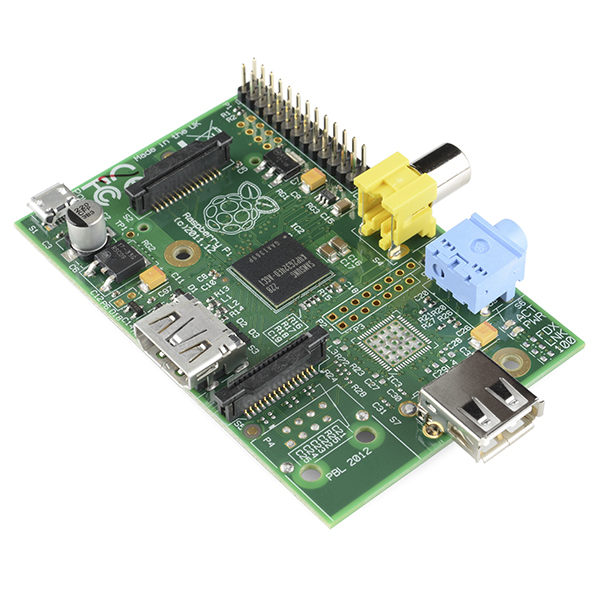
\includegraphics[scale = 1.5]{fig/Raspberry-Pi-1-modelo-A.jpg}
\caption{Raspberry Pi 1 modelo A}
\label{fig:raspberry-pi-1-modelo-a}
\end{figure}

\subsubsection{Raspberry Pi 1 modelo B}

\noindent También en 2012, la Raspberry Pi 1 modelo B apareció en el mercado trayendo el doble de memoria RAM que su predecesora, hasta los 512MB. Adicionalmente, también se le añadió un puerto USB más, y un conector RJ-45. Más tarde apareció el modelo B+, que incluía 4 puertos USB y usaba una tarjeta MicroSD, en lugar de la SD.

\subsubsection{Raspberry Pi 2 modelo B}

\noindent No fue hasta 2014 cuando hizo su aparición el siguiente modelo, la Raspberry Pi 2 modelo B, que cambió por primera vez el procesador de sus predecesoras, incorporando uno de 4 núcleos y aumentando su frecuencia hasta los 900MHz. La memoria RAM ascendió al doble de capacidad, llegando hasta 1GB. Además de todo eso, esta Raspberry Pi incluyó 40 pines GPIO y eliminó la conexión RCA. En la figura~\ref{fig:raspberry-pi-2-modelo-B} se muestra este modelo de Raspberry Pi.

\begin{figure}[tbp]
\centering
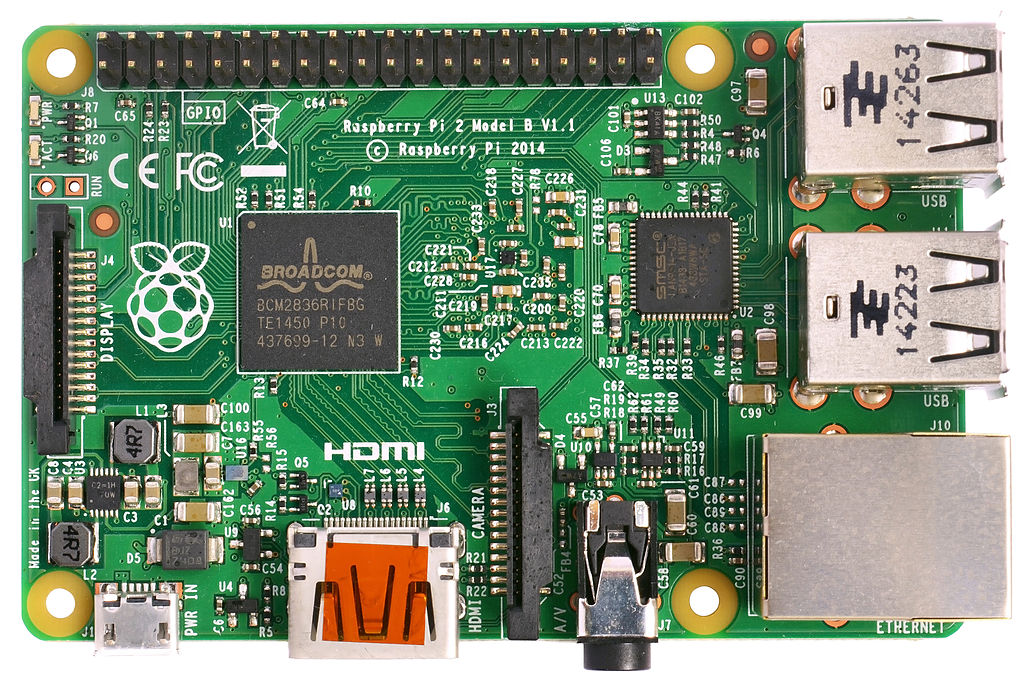
\includegraphics[scale = 1]{fig/Raspberry-Pi-2-modelo-B.jpg}
\caption{Raspberry Pi 2 modelo B}
\label{fig:raspberry-pi-2-modelo-B}
\end{figure}

\subsubsection{Raspberry Pi 3 modelo B}

\noindent Con nacimiento en 2016, la Raspberry Pi 3 modelo B llegó con un procesador nuevo y mejorado, que pasó de los 900MHz a 1.2GHz. Sin embargo, la principal novedad que traía este modelo de Raspberry Pi era la inclusión por primera vez de conexiones Wi-Fi y Bluetooth que no prescindían de adaptadores adicionales.

\subsubsection{Raspberry Pi 3 modelo B+}

\noindent A pesar de anunciarse como una actualización del modelo anterior, la Raspberry Pi 3 modelo B+ trajo diversas mejoras, entre las que se destacan las siguientes:
\begin{itemize}
\item{Mejora del procesador, que pasa de 1.2GHz a 1.4GHz}
\item{Incorporación de doble banda de 2.4GHz y 5GHz en la conectividad inalámbrica}
\item{El puerto Ethernet pasa de 100Mbits/s hasta los 300Mbits/s}
\item{Bluetooth 4.2}
\end{itemize}

\noindent Puede observarse la Raspberry Pi 3 modelo B+ en la figura~\ref{fig:raspberry-pi-3-modelo-Bplus}.

\begin{figure}[tbp]
\centering
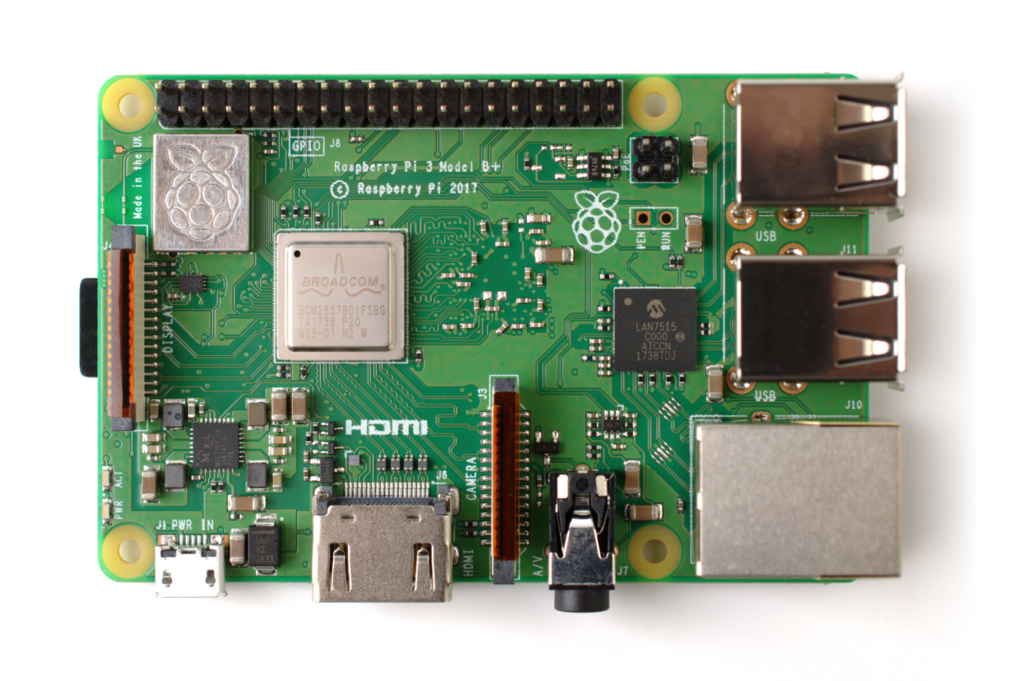
\includegraphics[scale = 0.3]{fig/Raspberry-Pi-3-modelo-B+.png}
\caption{Raspberry Pi 3 modelo B+}
\label{fig:raspberry-pi-3-modelo-Bplus}
\end{figure}

\subsubsection{Raspberry Pi 3 modelo A+}

\noindent Este modelo, que apareció en noviembre de 2018, no tenía por objeto mejorar las capacidades de sus predecesoras, si no presentar un precio más competitivo. Es por ello que, en este económico modelo contó con 512MB de RAM, un único puerto USB y eliminó la conexión RJ-45.

\subsubsection{Raspberry Pi 4 modelo B+}

\noindent Anunciada en junio de 2019, la Raspberry Pi 4 modelo B+ representa el prototipo más moderno durante la redacción de este trabajo de fin de grado. Este modelo cuenta con múltiples mejoras respecto a los modelos anteriores, entre las que pueden destacarse un procesador hasta 3 veces más eficiente que el anterior, la inclusión de una entrada USB 3.0 y el cambio de un puerto HDMI por dos puertos mini-HDMI. Este último modelo de Raspberry Pi se expone gráficamente en la figura~\ref{fig:raspberry-pi-4-modelo-B}.

\begin{figure}[tbp]
\centering
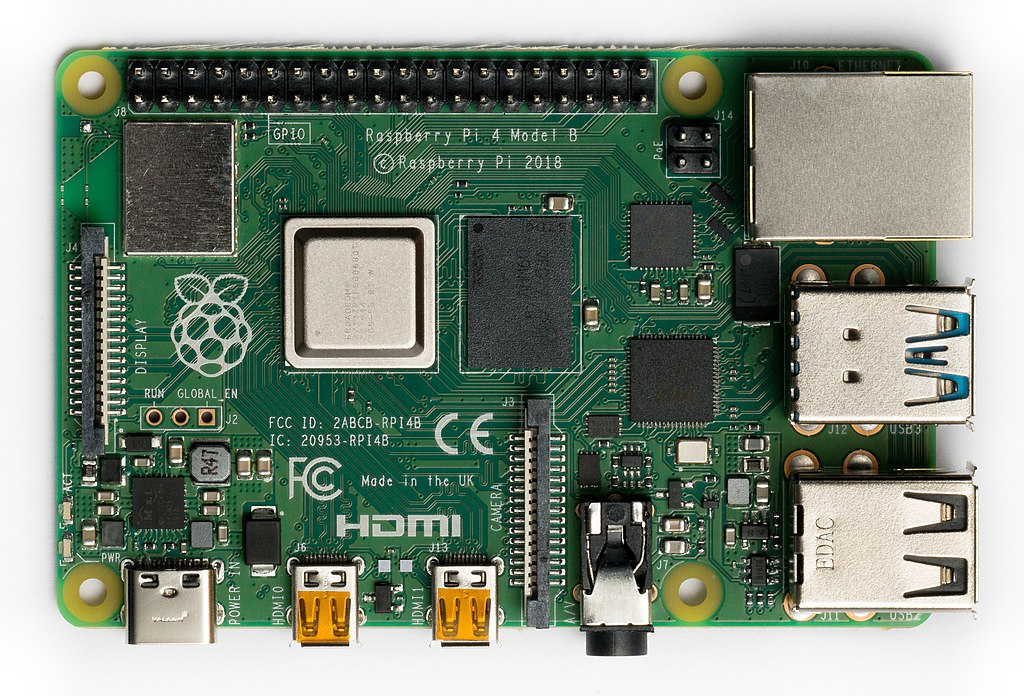
\includegraphics[scale = 0.3]{fig/Raspberry-Pi-4-modelo-B.jpg}
\caption{Raspberry Pi 4 modelo B}
\label{fig:raspberry-pi-4-modelo-B}
\end{figure}

Adicionalmente a los modelos básicos, la fundación Raspberry Pi también ha comercializado una gama de placas de menor coste y tamaño, llamadas Raspberry Pi Zero. Hasta la fecha, han aparecido tres modelos de este tipo de computadoras de bajo coste.

\subsubsection{Raspberry Pi Zero}

\noindent Hizo su aparición en 2015, y para entonces contaba ya con un procesador de 1GHz, 512MB de RAM. Debido a su diminuto tamaño, en lugar de usar los puertos HDMI y USB clásicos, hace uso de una entrada MiniHDMI y dos entradas MicroUSB. En la figura~\ref{fig:raspberry-pi-zero} se muestra esta mini computadora de bajo coste.

\begin{figure}[tbp]
\centering
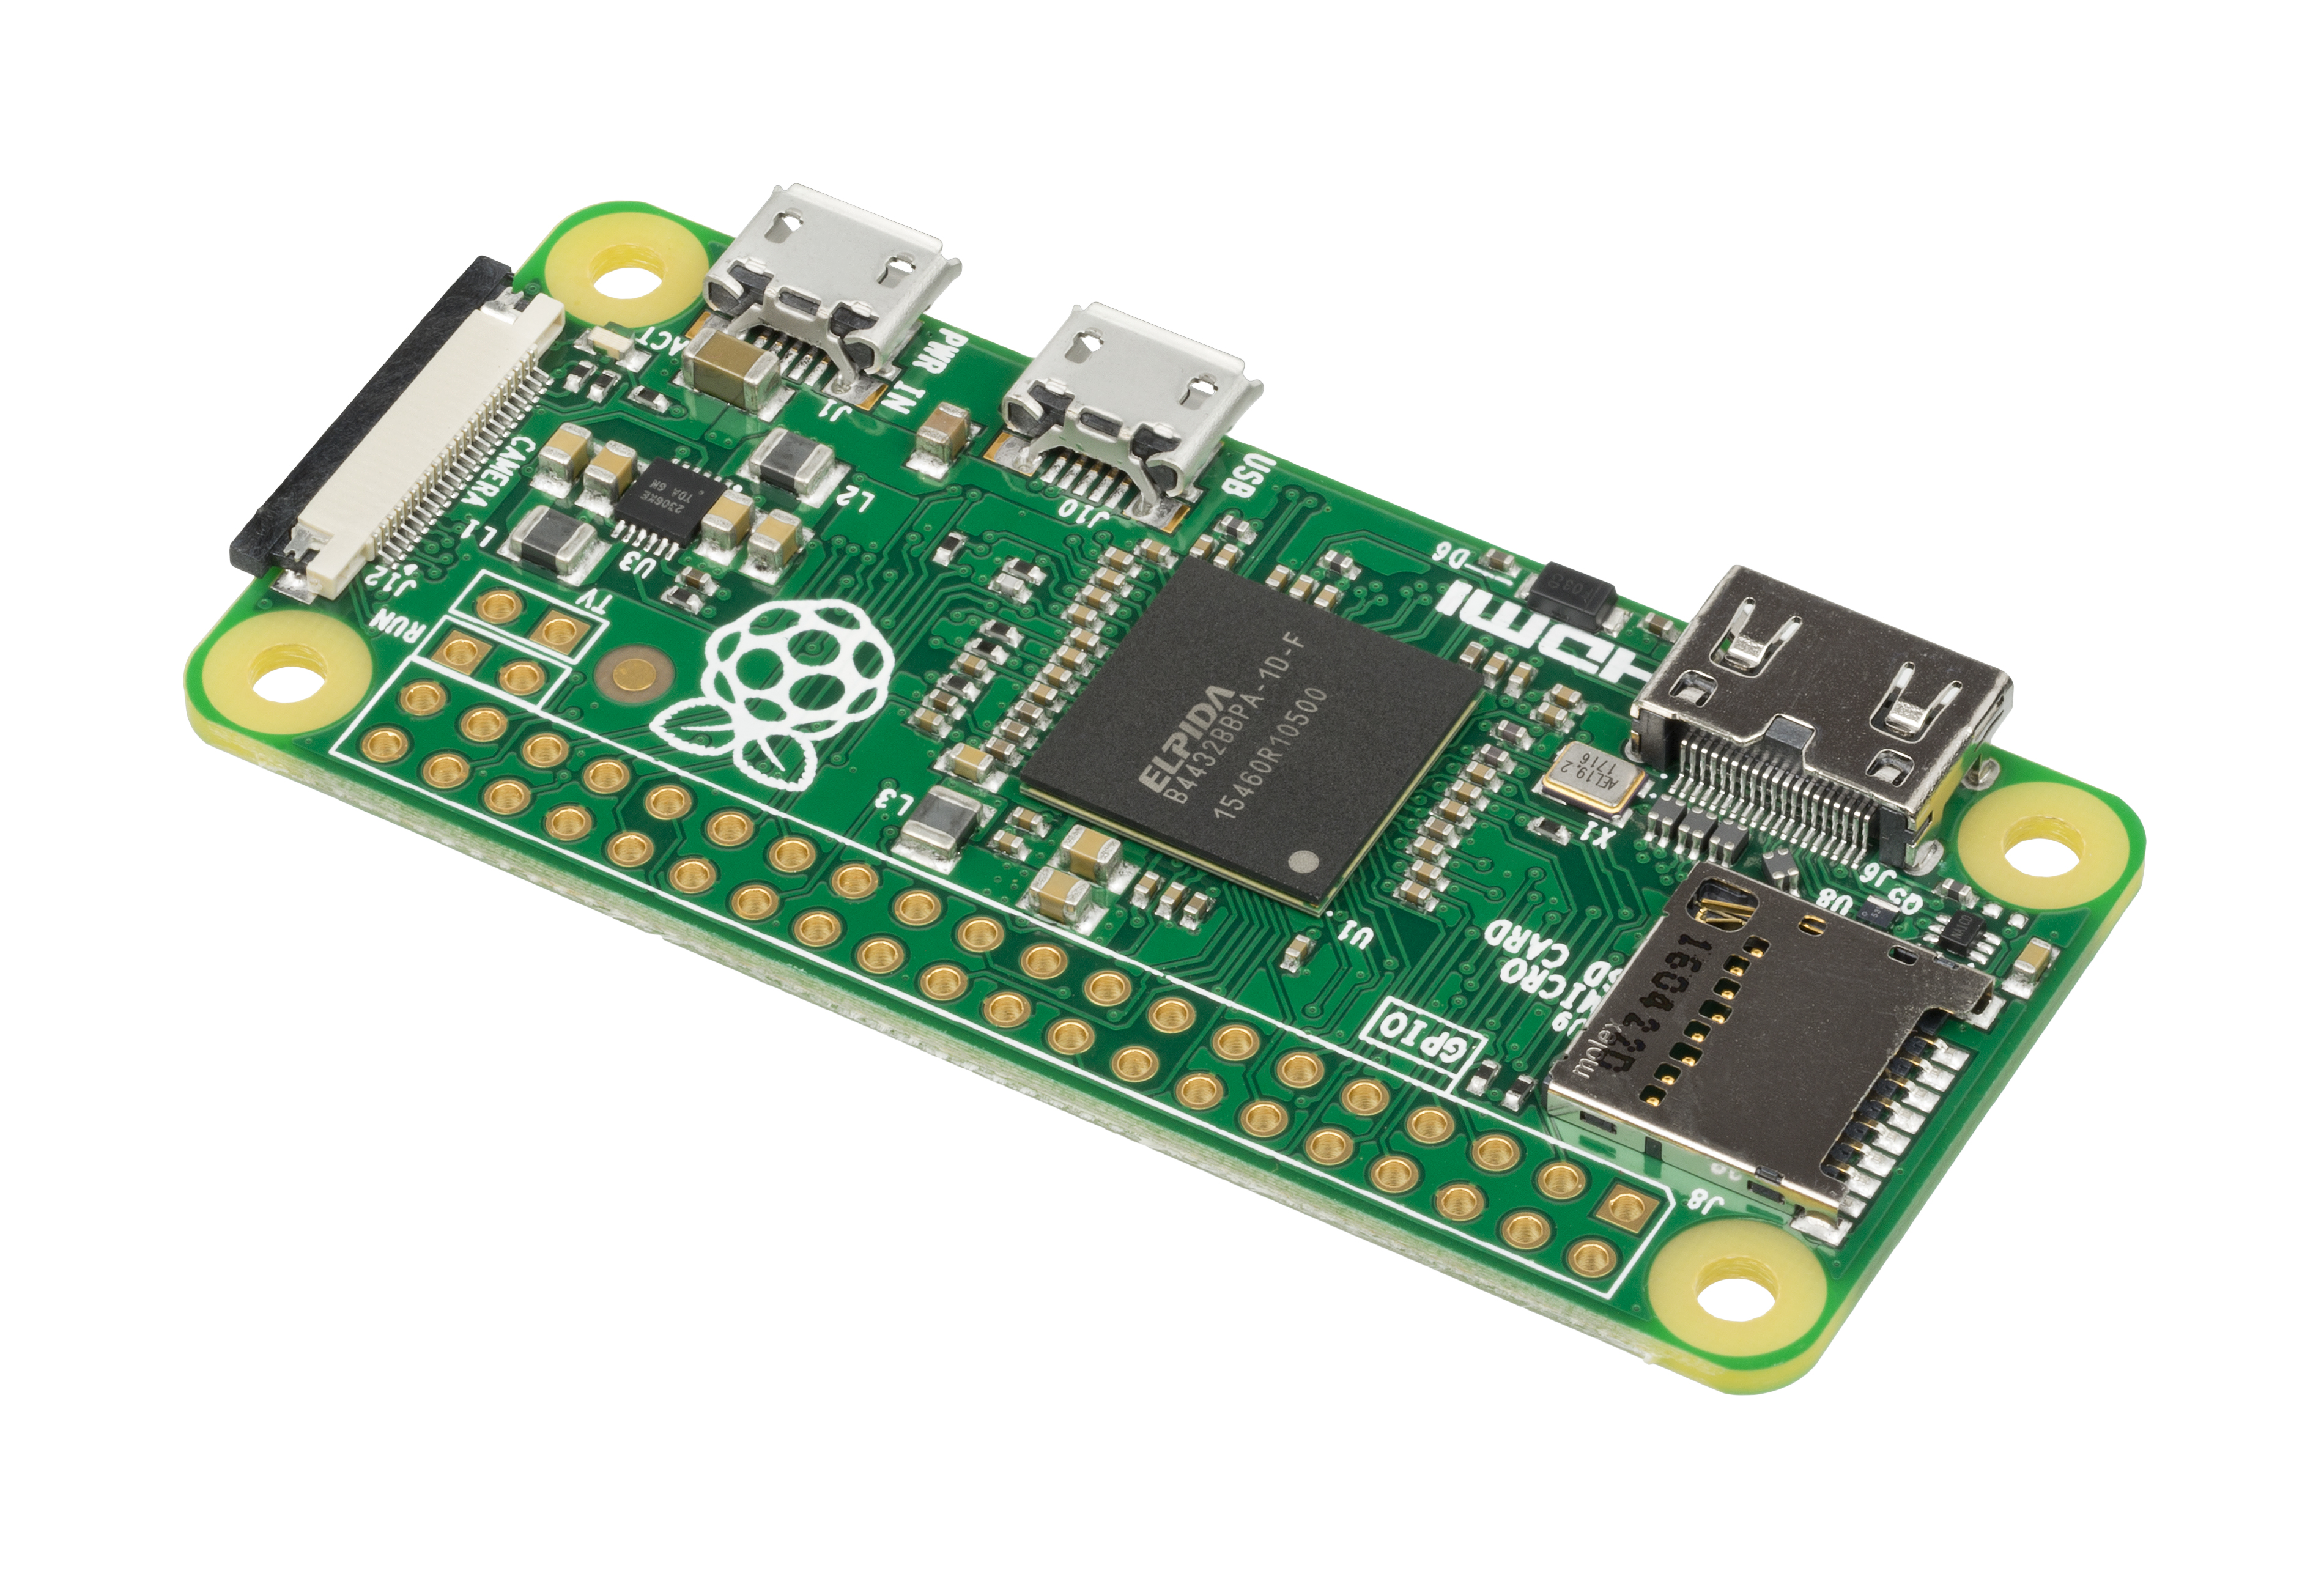
\includegraphics[scale = 0.24]{fig/Raspberry-Pi-Zero.jpg}
\caption{Raspberry Pi Zero}
\label{fig:raspberry-pi-zero}
\end{figure}

\subsubsection{Raspberry Pi Zero W}

\noindent La novedad que presenta este modelo respecto de su predecesora, es la inclusión de conexión por Bluetooth y Wi-Fi. Puede observarse este modelo de computadora en la figura~\ref{fig:raspberry-pi-zero-w}.

\begin{figure}[tbp]
\centering
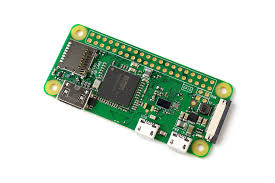
\includegraphics[scale = 1.2]{fig/Raspberry-Pi-Zero-W.jpg}
\caption{Raspberry Pi Zero W}
\label{fig:raspberry-pi-zero-w}
\end{figure}

\subsubsection{Raspberry Pi Zero WH}

\noindent Tan solo existe una diferencia entre este modelo y la Raspberry Pi  Zero W, y es la inclusión de un conector soldado a los 40 pines GPIO. Si quiere observarse la diferencia a nivel físico, no hay más que comparar esta computadora en la figura 1.7 con su predecesora en la figura~\ref{fig:raspberry-pi-zero-wh}.

\begin{figure}[tbp]
\centering
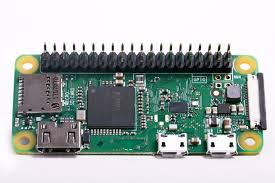
\includegraphics[scale = 0.8]{fig/Raspberry-Pi-Zero-WH.jpg}
\caption{Raspberry Pi Zero WH}
\label{fig:raspberry-pi-zero-wh}
\end{figure}

\subsection{Historia de los bots conversacionales}

\noindent En los tiempos que transcurren durante el desarrollo de este trabajo de fin de grado, los bots conversacionales parecen estar abriéndose camino a un público cada vez más amplío. Empresas como Microsoft, Google o Amazon apuestan por este tipo de tecnología, tratando de adaptarse a las necesidades de la gente con ayuda de algoritmos de inteligencia artificial.

Una buena forma de analizar la evolución de los bots, es por medio del test de Turing. En 1950, el matemático británico Alan Turing propuso un test a partir del cual se define la capacidad de un bot. La realización de dicho test consiste en ofrecer una serie de respuestas a un humano, que tendrá que decidir si estas han sido proporcionadas por otro humano o por una computadora.

Inspirado por el trabajo de Turing, el alemán Joseph Weizenbaum, desarrolló en 1966 el que sería el primer bot de la historia, al cual bautizó con el nombre de "ELIZA". Este bot consistía en un algoritmo que trataba de reconocer ciertas palabras clave, a partir de las cuales, ofrecía respuestas lógicas. Durante las pruebas conversacionales ejercidas entre humanos y ELIZA, múltiples personas creyeron estar hablando con un humano y compartieron con este bot detalles íntimos, haciendo de esta manera que ELIZA superara, a nivel teórico, el test de Turing.

De esta manera, en el 2000, apoyándose en la base establecida por sus predecesores, apareció SmarterChild, un bot capaz de procesar y entender de cierta manera el lenguaje, ofreciendo respuestas que permitían ayudar al usuario, con temas tan diversos como previsiones de meteorología o entradas de cine. SmarterChild era además compatible con plataformas de mensajería conocidas como MSN Messenger, y estableció por tanto un primer contacto entre el mundo de los bots conversacionales y el público general.

Desde entonces, la propagación de los bots, tanto de voz como escritos, se ha extendido en múltiples campos y plataformas. Desde los asistentes virtuales como Alexa y Google Home, hasta los múltiples bots de Telegram\cite{elenasantos2018} que permiten, entre otras muchas cosas, obtener imágenes de cualquier cosa con solo pedirlas o conocer la predicción meteorológica.

A finales del año 2018 ya se encontraban en funcionamiento\cite{albertoiglesiasfraga2019} más de 2.500 millones de asistentes virtuales, lo cual da muestra del estado de buena salud por el que pasa este tipo de tecnología.

\chapter{Objetivos}
\label{ch:objetivos}

\noindent El objeto principal de este trabajo de fin de grado es el de automatizar por completo la recepción de los turistas en las viviendas de uso turístico, de manera que los propietarios de las mismas no tengan que dedicar su tiempo a esta tarea. Para la llevar a cabo esta empresa, el objetivo principal se desglosa en otros más pequeños que trabajarán en conjunto. A continuación se identifican y explican cada uno de los objetivos que se han considerado:

\section{Circuito electrónico capaz de abrir una cerradura eléctrica} 
\label{sec:circuito-electronico-capaz-de-abrir-una-cerradura-electrica}

\noindent Para poder abrir la puerta a los clientes en su llegada, es necesario que el circuito sea capaz de abrir la puerta. Este objetivo se alcanzará una vez que, a partir de una señal de 3 voltios emitida por la Raspberry Pi Zero W, se proceda a activar la apertura de una cerradura eléctrica. Para ello se hará uso de los materiales que resulten convenientes, como relés, transformadores, cableado, etc.

\section{Programa para apertura de la vivienda desde Telegram} 
\label{sec:programa-que-atienda-las-peticiones-de-apertura-desde-telegram}

\noindent El presente objetivo estará completado en el momento en que el turista, al llegar a la vivienda de uso turístico, tenga la posibilidad de realizar la apertura de la vivienda desde la aplicación de Telegram.

\section{Panel de administración desde Telegram} 
\label{sec:creacion-de-un-panel-de-administracion-desde-telegram}

\noindent Como administrador, la persona o personas que gestionen la vivienda tendrán la posibilidad de realizar distintas actividades desde la propia plataforma de Telegram. Este objetivo se habrá alcanzado en el momento en que, por medio de un programa integrado en la Raspberry Pi, el administrador sea capaz de realizar las siguientes operaciones:

\begin{itemize}
\item Consultar las reservas existentes. El anfitrión tendrá la posibilidad de consultar todas las reservas que contenga el sistema.
\item Crear nuevas reservas. El anfitrión podrá crear reservas para los días que considere convenientes, desde un panel de gestión implantado en la propia aplicación de Telegram.
\item Anular reservas. De igual manera, el anfitrión tendrá la posibilidad de cancelar aquellas reservas que considere convenientes.
\item Por último, el panel de administración para el anfitrión incluirá la posibilidad de realizar la apertura de las puertas de forma automática.
\end{itemize}

\section{Automatización de nuevas reservas} 
\label{sec:automatizacion-de-nuevas-reservas}

\noindent Con el fin de que el propietario de la vivienda de uso turístico pueda automatizar el proceso de atención de los clientes, la Raspberry Pi integrará un programa  en el que se gestionarán todas las nuevas reservas que se produzcan de la vivienda, de manera que permitirá la entrada a los clientes una vez que estos se identifiquen a través de su número de reserva.

\section{Automatización de cancelaciones de reservas} 
\label{sec:automatizacion-de-cancelaciones-de-reservas}

\noindent En la mayoría de plataformas de alquiler vacacional, como Booking, Airbnb, Homeaway, etc. Los clientes tienen la posibilidad de realizar cancelaciones. Por lo tanto, esto es algo que se debe tener en cuenta a la hora de automatizar el proceso de reservas y recepción de clientes. Para tal efecto se integrará un programa en la Raspberry Pi que recibirá las cancelaciones de los clientes, y lo incluirá en el sistema, de manera que esas personas no tendrán acceso a la vivienda por medio del número de reserva que obtuvieron antes de su cancelación.

\section{Diseño en tres dimensiones para contener el circuito} 
\label{sec:creacion-de-un-diseño-en-tres-dimensiones-para-contener-el-circuito}

\noindent Con el fin de mejorar la seguridad del sistema, así como su aspecto visual, se procederá a crear un diseño en tres dimensiones donde se contendrá todo el circuito electrónico.

Este diseño deberá permitir su instalación en la pared, por medio de tornillería o por medio de adhesivos, y proporcionará una sujeción firme de los elementos que se encuentren en su interior.

También integrará la posibilidad de incluir un candado que asegure su cierre, de manera que se trate de evitar la manipulación indeseada por parte de otros usuarios.


\section{Sistema de alarma ante posibles manipulaciones} 
\label{sec:sistema-de-alarma-ante-posibles-manipulaciones}

\noindent Todas las medidas de seguridad que se tomen serán de gran ayuda para crear confianza en aquellos propietarios que quieran hacer uso de este sistema. Si la Raspberry Pi trabajase de forma manipulada por algún usuario malintencionado, podría significar un problema importante de seguridad. Es por ello que se integrará en la placa un programa que permitirá advertir al administrador principal, por medio de un correo electrónico, en caso de que alguien haya abierto la caja donde se encuentra. De esta manera se le permitirá conocer la situación y actuar en consecuencia.

\section{Sistema de alarma ante interrupciones} 
\label{sec:sistema-de-alarma-ante-interrupciones}

\noindent Un apagón, una caída de internet o un fallo interno de la Raspberry Pi, podrían provocar en un momento determinado una interrupción en el trabajo de la misma. Para que el administrador principal pueda ser conocedor de ello, y actuar en consecuencia, se incluirá un programa con el que se le avisará de lo sucedido a través de un correo electrónico.

\chapter{Contribuciones}
\label{ch:contribuciones}

Las contribuciones que se derivan de este trabajo de fin de grado, por parte del autor, son las siguientes:
\begin{itemize}
\item Desarrollo de un algoritmo, aplicado al mercado de las viviendas de uso turístico, capaz de recibir las reservas de clientes por medio de un correo electrónico, analizar el contenido del mismo, y de esta manera organizar todas las entradas en la vivienda. Se hace uso del lenguaje de programación python, aplicado en una computadora Raspberry Pi Zero W, con la librería SMPTLIB.
\item Desarrollo de un algoritmo, aplicado al mercado de las viviendas de uso turístico, capaz de recibir la cancelación de reservas por parte de los clientes, a través de un correo electrónico, analizar el contenido del mismo, y de esta manera organizar todas las entradas en la vivienda. Se hace uso del lenguaje de programación python, aplicado en una computadora Raspberry Pi Zero W, con la librería SMPTLIB.
\item Creación de un panel de control para realizar la administración de una vivienda de uso turístico a través de la aplicación de mensajería instantánea "Telegram". Se hace uso del lenguaje de programación python, aplicado en una computadora Raspberry Pi Zero W, con la librería TelegramBotApi.
\item Creación de un panel de usuario final para los clientes de viviendas de uso turístico, a partir del cual se les permite acceder a la vivienda, una vez que han sido identificados. Se hace uso del lenguaje de programación python, aplicado en una computadora Raspberry Pi Zero W, con la librería TelegramBotApi.
\item Circuito electrónico, de bajo coste, capaz de realizar la apertura de cerraduras eléctricas por medio de una Raspberry Pi Zero W. Se hace uso de una computadora Raspberry Pi Zero W, transformadores, un relé, un portero automático \textbf{FERMAX (FALTA INDICAR MODELO} y el cableado pertinente.
\item Sistema de seguridad para evitar posibles manipulaciones del circuito electrónico encargado de gestionar las entradas de viviendas de uso turístico. Se hace uso del lenguaje de programación python en una computadora Raspberry Pi Zero W, una impresora 3D, un candado de seguridad, un sensor de ultrasonido HC-SR04 y el cableado pertinente.
\end{itemize}
\chapter{Procedimiento}
\label{ch:procedimiento}

En el desarrollo de este TFG se ha utilizado una metodología ágil basada en \emph{Scrum}~\cite{scrumguide}, definida por el director.  El trabajo se ha dividido en iteraciones de dos semanas denominadas \emph{sprints}.  Las unidades de trabajo se presentan en forma de historias de usuario (\emph{user stories}) que definen mini-proyectos de muy corta duración que aportan valor al proyecto.  Es decir, cada historia de usuario cumple o ayuda a cumplir alguno de los objetivos.  Medir el valor percibido corresponde al propietario del producto (\emph{Product Owner}), que participa activamente en la planificación del proceso priorizando las unidades de trabajo.

La utilización de una metodología ágil permite equilibrar la cantidad de trabajo y los objetivos alcanzados.  Los 12 créditos ECTS del TFG se reparten según el criterio del director para que los resultados aporten el máximo valor posible, incluso en presencia de imprevistos.

\section{Diferencias con Scrum}

\emph{Scrum} es una metodología estrictamente centrada en el cliente.  El cliente es el responsable de priorizar y, en cierto modo, planificar las iteraciones.  Esto garantiza que la ejecución del proyecto responde al máximo con las expectativas del cliente, aún cuando los imprevistos impidan alcanzar alguno de los objetivos iniciales.  Esta característica de \emph{Scrum} es la única que se ha intentado mantener inalterada.  Sin embargo, el TFG es un proyecto individual, lo que ha requerido modificar significativamente otros aspectos de la metodología.

\subsection{Roles}

La única remuneración que se obtiene con la ejecución de un TFG es la calificación de los distintos aspectos (anteproyecto, valoración del director, valoración del tribunal, etc.).  Por tanto, el cliente del TFG se compone por el director y el tribunal de la defensa.  Desgraciadamente no es posible conocer a priori el tribunal.  Por este motivo el director es el único representante del cliente en el proceso de desarrollo (\emph{Product Owner}).

El TFG debe ser realizado de manera individual.  Por tanto, el equipo de trabajo (\emph{Team Member}) se compone exclusivamente por el autor.

La labor de dirección del TFG se asimila a la de dirección del proyecto y, por tanto, el director también actúa como coordinador del proceso, o \emph{Scrum Master}.  Nótese que hay dos roles representados por la misma persona.  Desde un punto de vista purista esto implica que puede haber conflicto de intereses y los intereses del cliente pueden estar insuficientemente representados.  Es una limitación extrínseca, que no es posible solucionar con el proceso actual.  Aún así, el uso de una metodología ágil centrada en el cliente debe mejorar el alineamiento de intereses cuando sobrevienen problemas que afectan o pueden afectar a la consecución de alguno de los objetivos iniciales.

\subsection{Historias de usuario}

\emph{Scrum}, como la mayoría de los métodos ágiles, está enfocada al desarrollo de proyectos en entornos de alta incertidumbre por equipos multidisciplinares bien formados.  El desarrollo de un TFG, al tratarse de un primer proyecto profesional, también está sometido a gran cantidad de incertidumbre.  Sin embargo, no siempre se cuenta con la formación previa necesaria para abordar todos los problemas.  Esto implica que, en ocasiones, se necesita aprender o leer, sin repercusión medible en el valor percibido por el \emph{Product Owner}.  En esos casos se planifican unidades de trabajo que no corresponden estrictamente a historias de usuario en el sentido de Scrum.  Se ha intentado mantener al mínimo este tipo de historias de usuario para tener el proceso lo más controlado posible.

Puntualmente ha sido necesario planificar historias de usuario que solo pretenden explorar opciones.  Este tipo de historias de usuario están contempladas en \emph{Scrum}, se denominan \emph{spikes}.  Sin embargo, en la ejecución de este TFG se ha procurado reducir al mínimo para que la exploración de alternativas no domine en el tiempo dedicado al TFG.

\subsection{Planificación de sprints}

Para la planificación y el seguimiento se ha utilizado un tablero \href{http://trello.com}{Trello}.  Los tableros Trello permiten agrupar tarjetas en una serie de listas con nombre.  Se ha utilizado el esquema propuesto en~\cite{andrewlittlefield2018}.

El autor ha sido responsable de añadir la mayoría de las historias de usuario a la lista \emph{Backlog}.  Se trata de un proceso continuo, durante toda la ejecución del proyecto.  El director, como \emph{product owner}, prioriza las historias, moviendo las tarjetas dentro de la lista \emph{Backlog}.  Justo antes de cada iteración se realiza una reunión presencial o virtual para revisar la iteración pasada y planificar la siguiente iteración.

Usando la técnica de \emph{planning poker} (ver~\cite{scrumguide}) se dimensionan las historias de usuario en días de trabajo.  Esta técnica consiste en un proceso de generación de consenso entre el autor y el director sobre el tiempo requerido para la ejecución de cada historia de usuario.  La unidad empleada ha sido de un día.

El director, como \emph{product owner} traslada las tarjetas correspondientes a las primeras historias de la lista \emph{Backlog} a la lista \emph{ToDo} hasta completar los 10 días de trabajo de la iteración.

\subsection{Flujo de trabajo}

El flujo de trabajo diario del autor corresponde a la siguiente secuencia:

\begin{itemize}
    \item Dentro de la lista \emph{ToDo} puede elegirse cualquier tarjeta para trabajar en ella.  Antes de comenzar el trabajo se arrastra la tarjeta a la lista \emph{Doing}.  Esto proporciona información en tiempo real al director del progreso de la iteración.
    
    \item Al terminar una historia de usuario la tarjeta correspondiente se arrastra a la lista \emph{QC} (quality control).
    
    \item El director, como \emph{Scrum Master}, revisa que la historia está realmente acabada y, si así es, la traslada a la lista \emph{Done}. En caso contrario la traslada a la lista \emph{Doing} otra vez, añadiendo un comentario que lo justifica.

    \item Si en el transcurso del trabajo se encuentra un obstáculo que impide progresar con una historia, se traslada a la lista \emph{Blocked}, añadiendo un comentario que lo justifica.
\end{itemize}

En todo momento es posible ver el estado global de ejecución del proyecto.  Al finalizar, la lista \emph{Done} contiene todas las historias de usuario ejecutadas por orden de terminación.  Y las listas \emph{Blocked} y \emph{Backlog} contienen (en este orden) todas las historias de usuario que corresponderían a trabajo futuro, ya priorizadas por el director.

\subsection{Herramientas de ayuda}

El proceso de desarrollo está fuertemente ligado a la herramienta \href{https://trello.com/}{Trello}.  Se trata de una herramienta colaborativa en línea, que permite mantener una serie de tarjetas agrupadas en listas con nombre.  Cada tarjeta puede tener un título, una descripción, un conjunto de adjuntos, y un conjunto de comentarios.  Trello se ha usado con éxito en la planificación de proyectos de nivel de complejidad muy variable.  Por ejemplo, Epic Games utiliza un tablero Trello para planificar las características a incorporar a cada nueva versión de Unreal Engine.  Por otro lado, un problema de Trello es el manejo limitado de la historia de modificaciones en las tarjetas y en los movimientos entre listas de tarjetas.  Esto dificulta en cierto modo el seguimiento de los cambios y, sobre todo, la corrección de errores en el proceso.  Por este motivo, Trello solo se ha empleado en la coordinación del trabajo, mientras que toda la gestión de cambios se ha delegado en otra herramienta.

Todo el proyecto ha sido gestionado desde su inicio con una herramienta de control de versiones distribuido en un repositorio público de GitHub, disponible en \thegitrepo.  Cada vez que se completa con éxito una historia de usuario se notifica mediante un comentario en la tarjeta correspondiente.  Este comentario tan solo contiene el identificador del paquete de cambios (\emph{commit}) que da por concluida la historia.  Todos los \emph{stakeholders} pueden consultar la evolución del proyecto en todo momento desde la propia página del repositorio.

\begin{figure}[tbp]
\centering
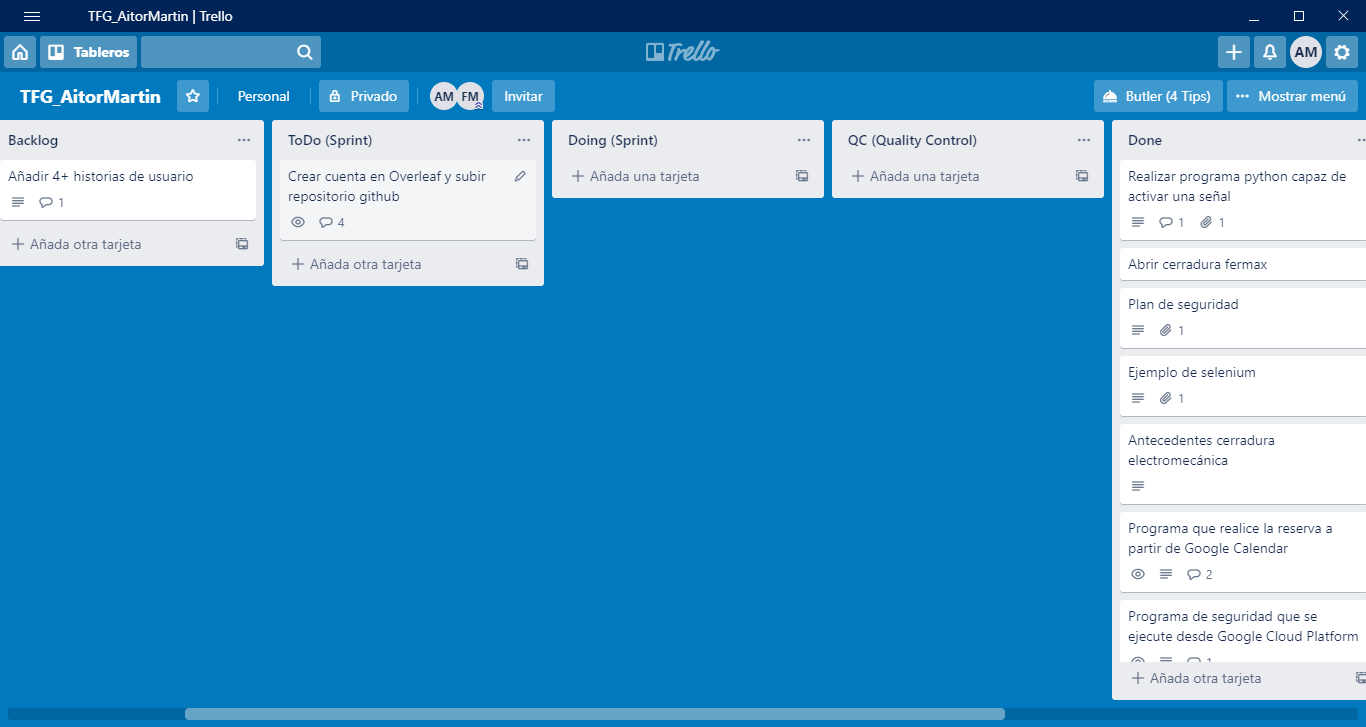
\includegraphics[scale = 0.4]{fig/tableto-trello.PNG}
\caption{Tableto trello utilizado en el desarrollo de este trabajo de fin de grado}
\label{fig:tableto-de-trello}
\end{figure}
\chapter{Resultados}
\label{ch:resultados}

La propia estructuración de los objetivos definidos para este trabajo de fin de grado servirá como base para la exposición de los resultados. De esta manera, se obtendrá un enfoque global, y a la vez, detallado, de cada una de las partes que componen el proyecto.

Para ello, al igual que en puntos anteriores, esta sección se dividirá en tres partes bien diferenciadas: Desarrollo del circuito electrónico, diseño de algoritmos y programación y tareas orientadas a la seguridad del dispositivo.
\section{Construcción del circuito electrónico}

La construcción del circuito electrónico definida en la fase de planificación contaba con dos objetivos principales, que eran los de realizar las conexiones necesarias para el correcto funcionamiento del dispositivo y fijar los elementos de manera segura y firme.

\begin{figure}[tbp]
\centering
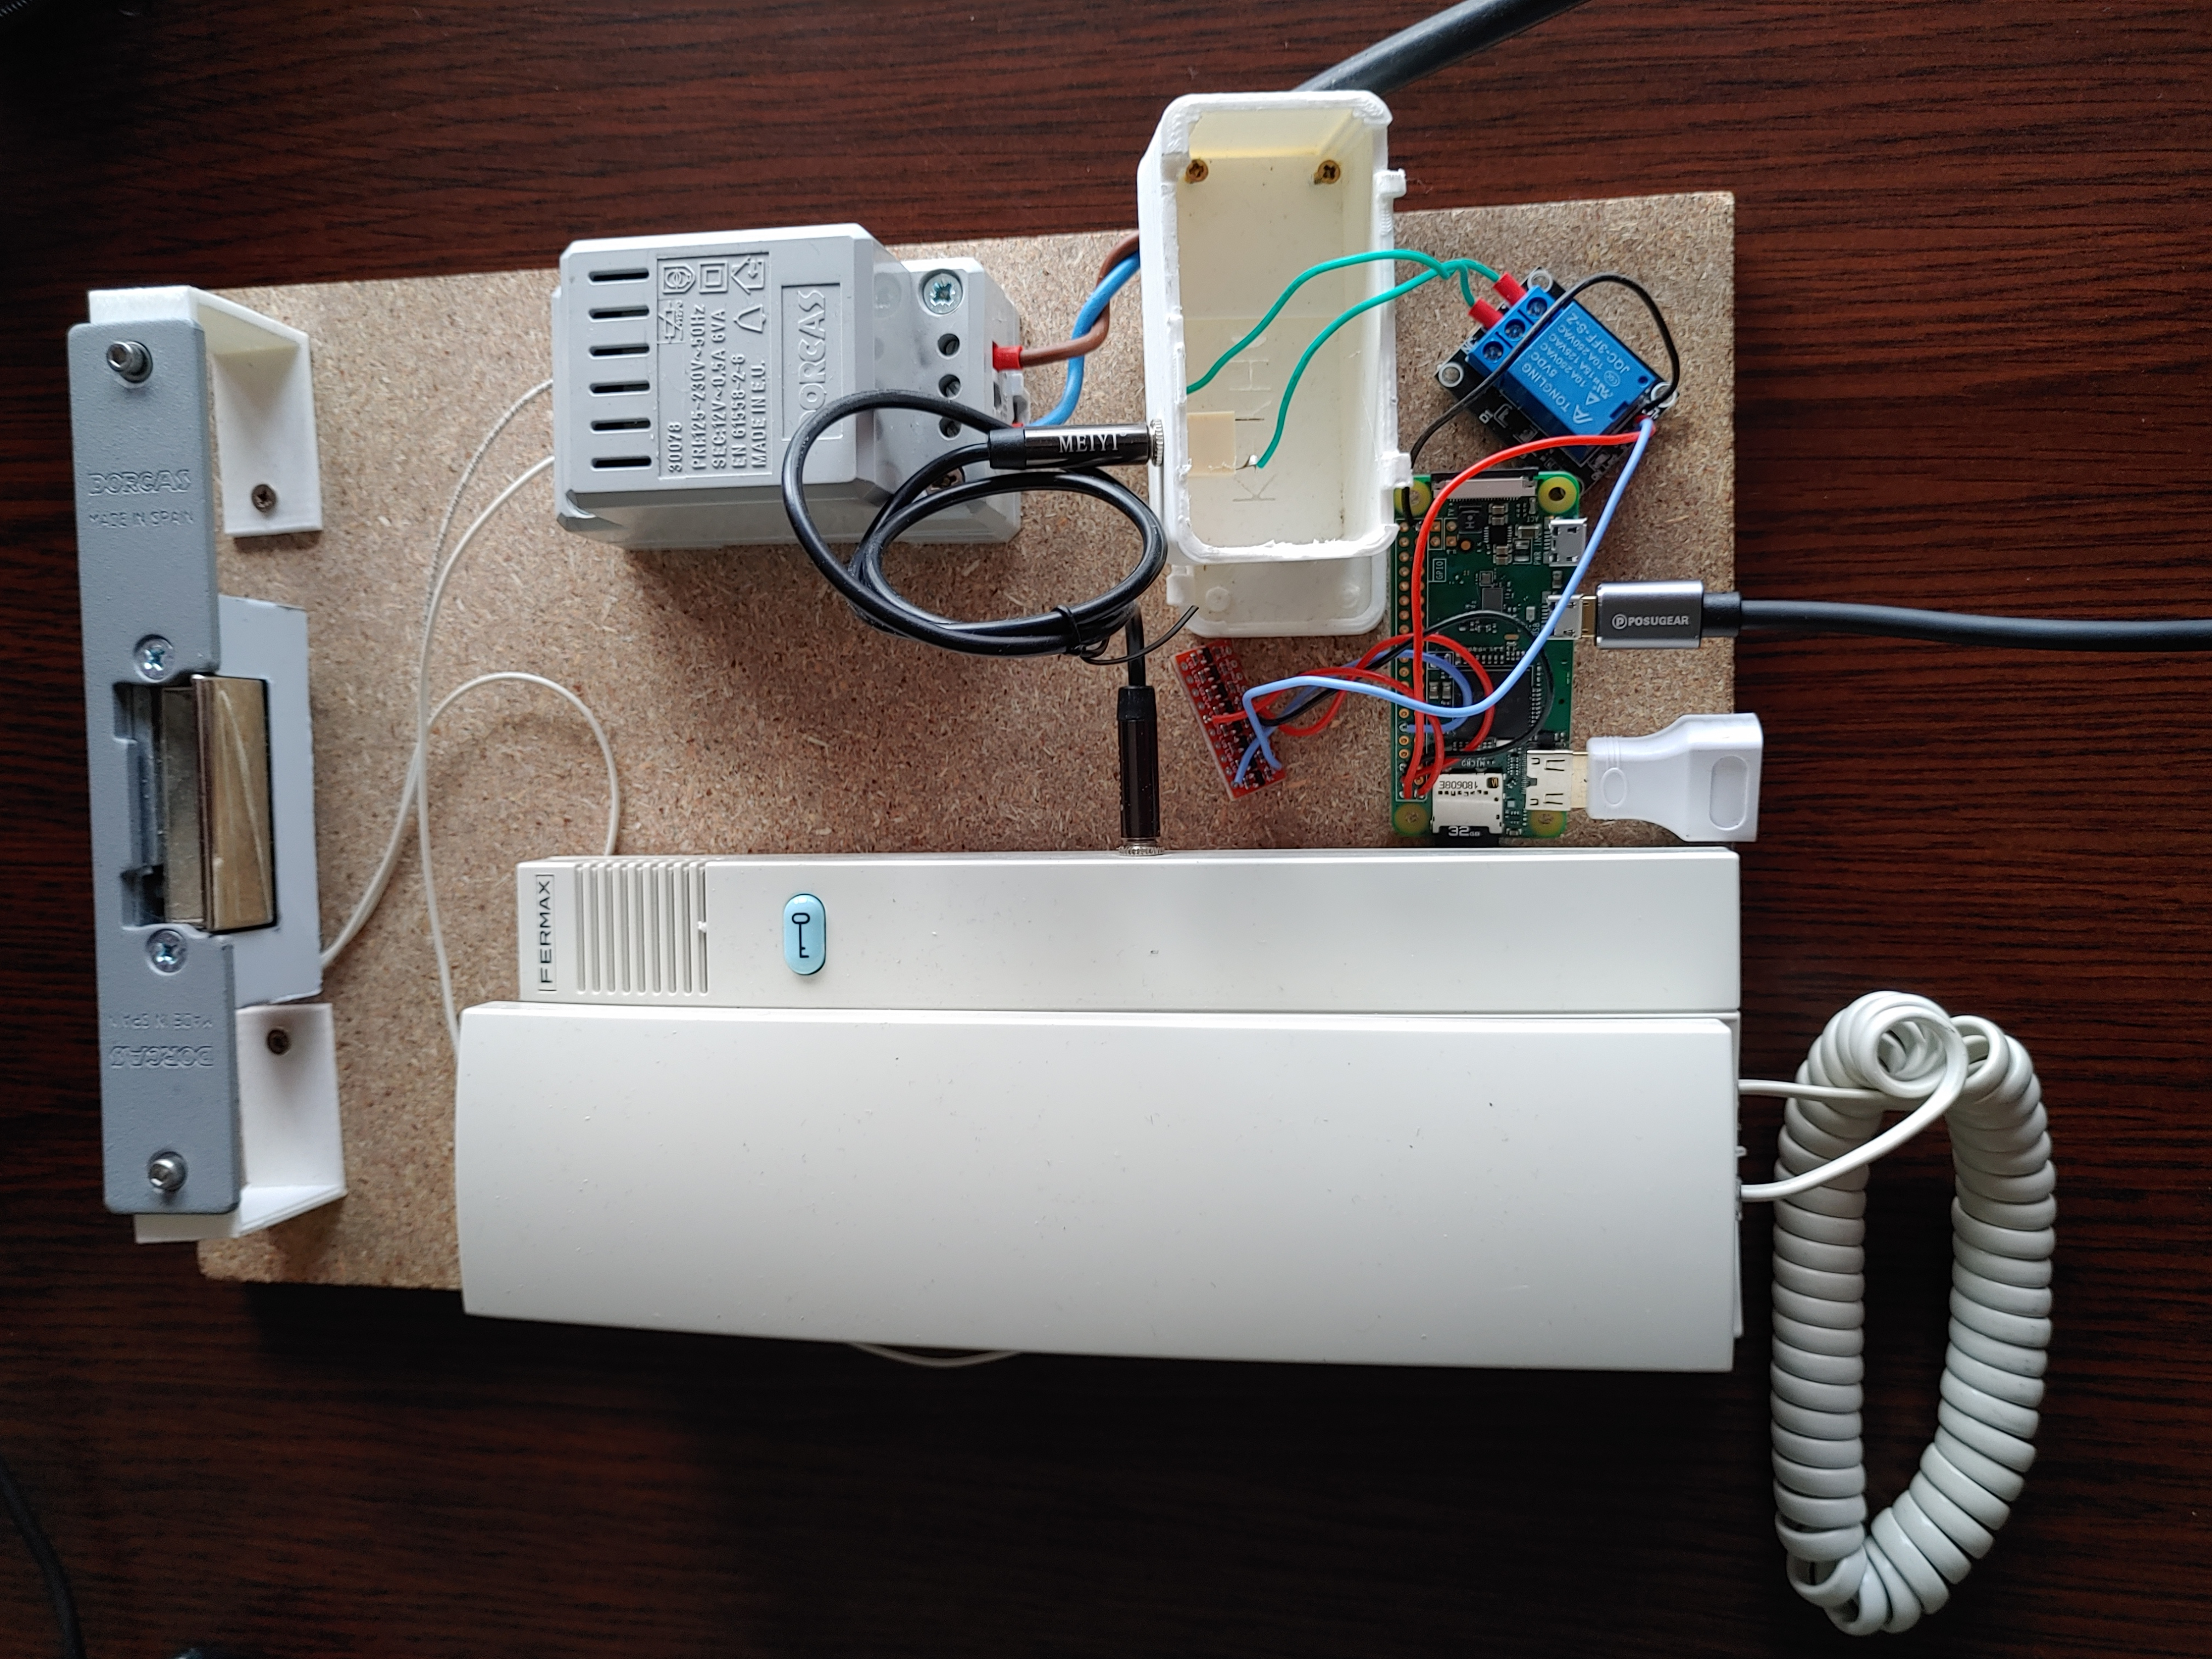
\includegraphics[scale = 0.1]{Prototipo_Completo.jpg}
\caption{Prototipo completo con todas las conexiones}
\label{fig:prototipo-completo}
\end{figure}
\begin{figure}[tbp]
\centering
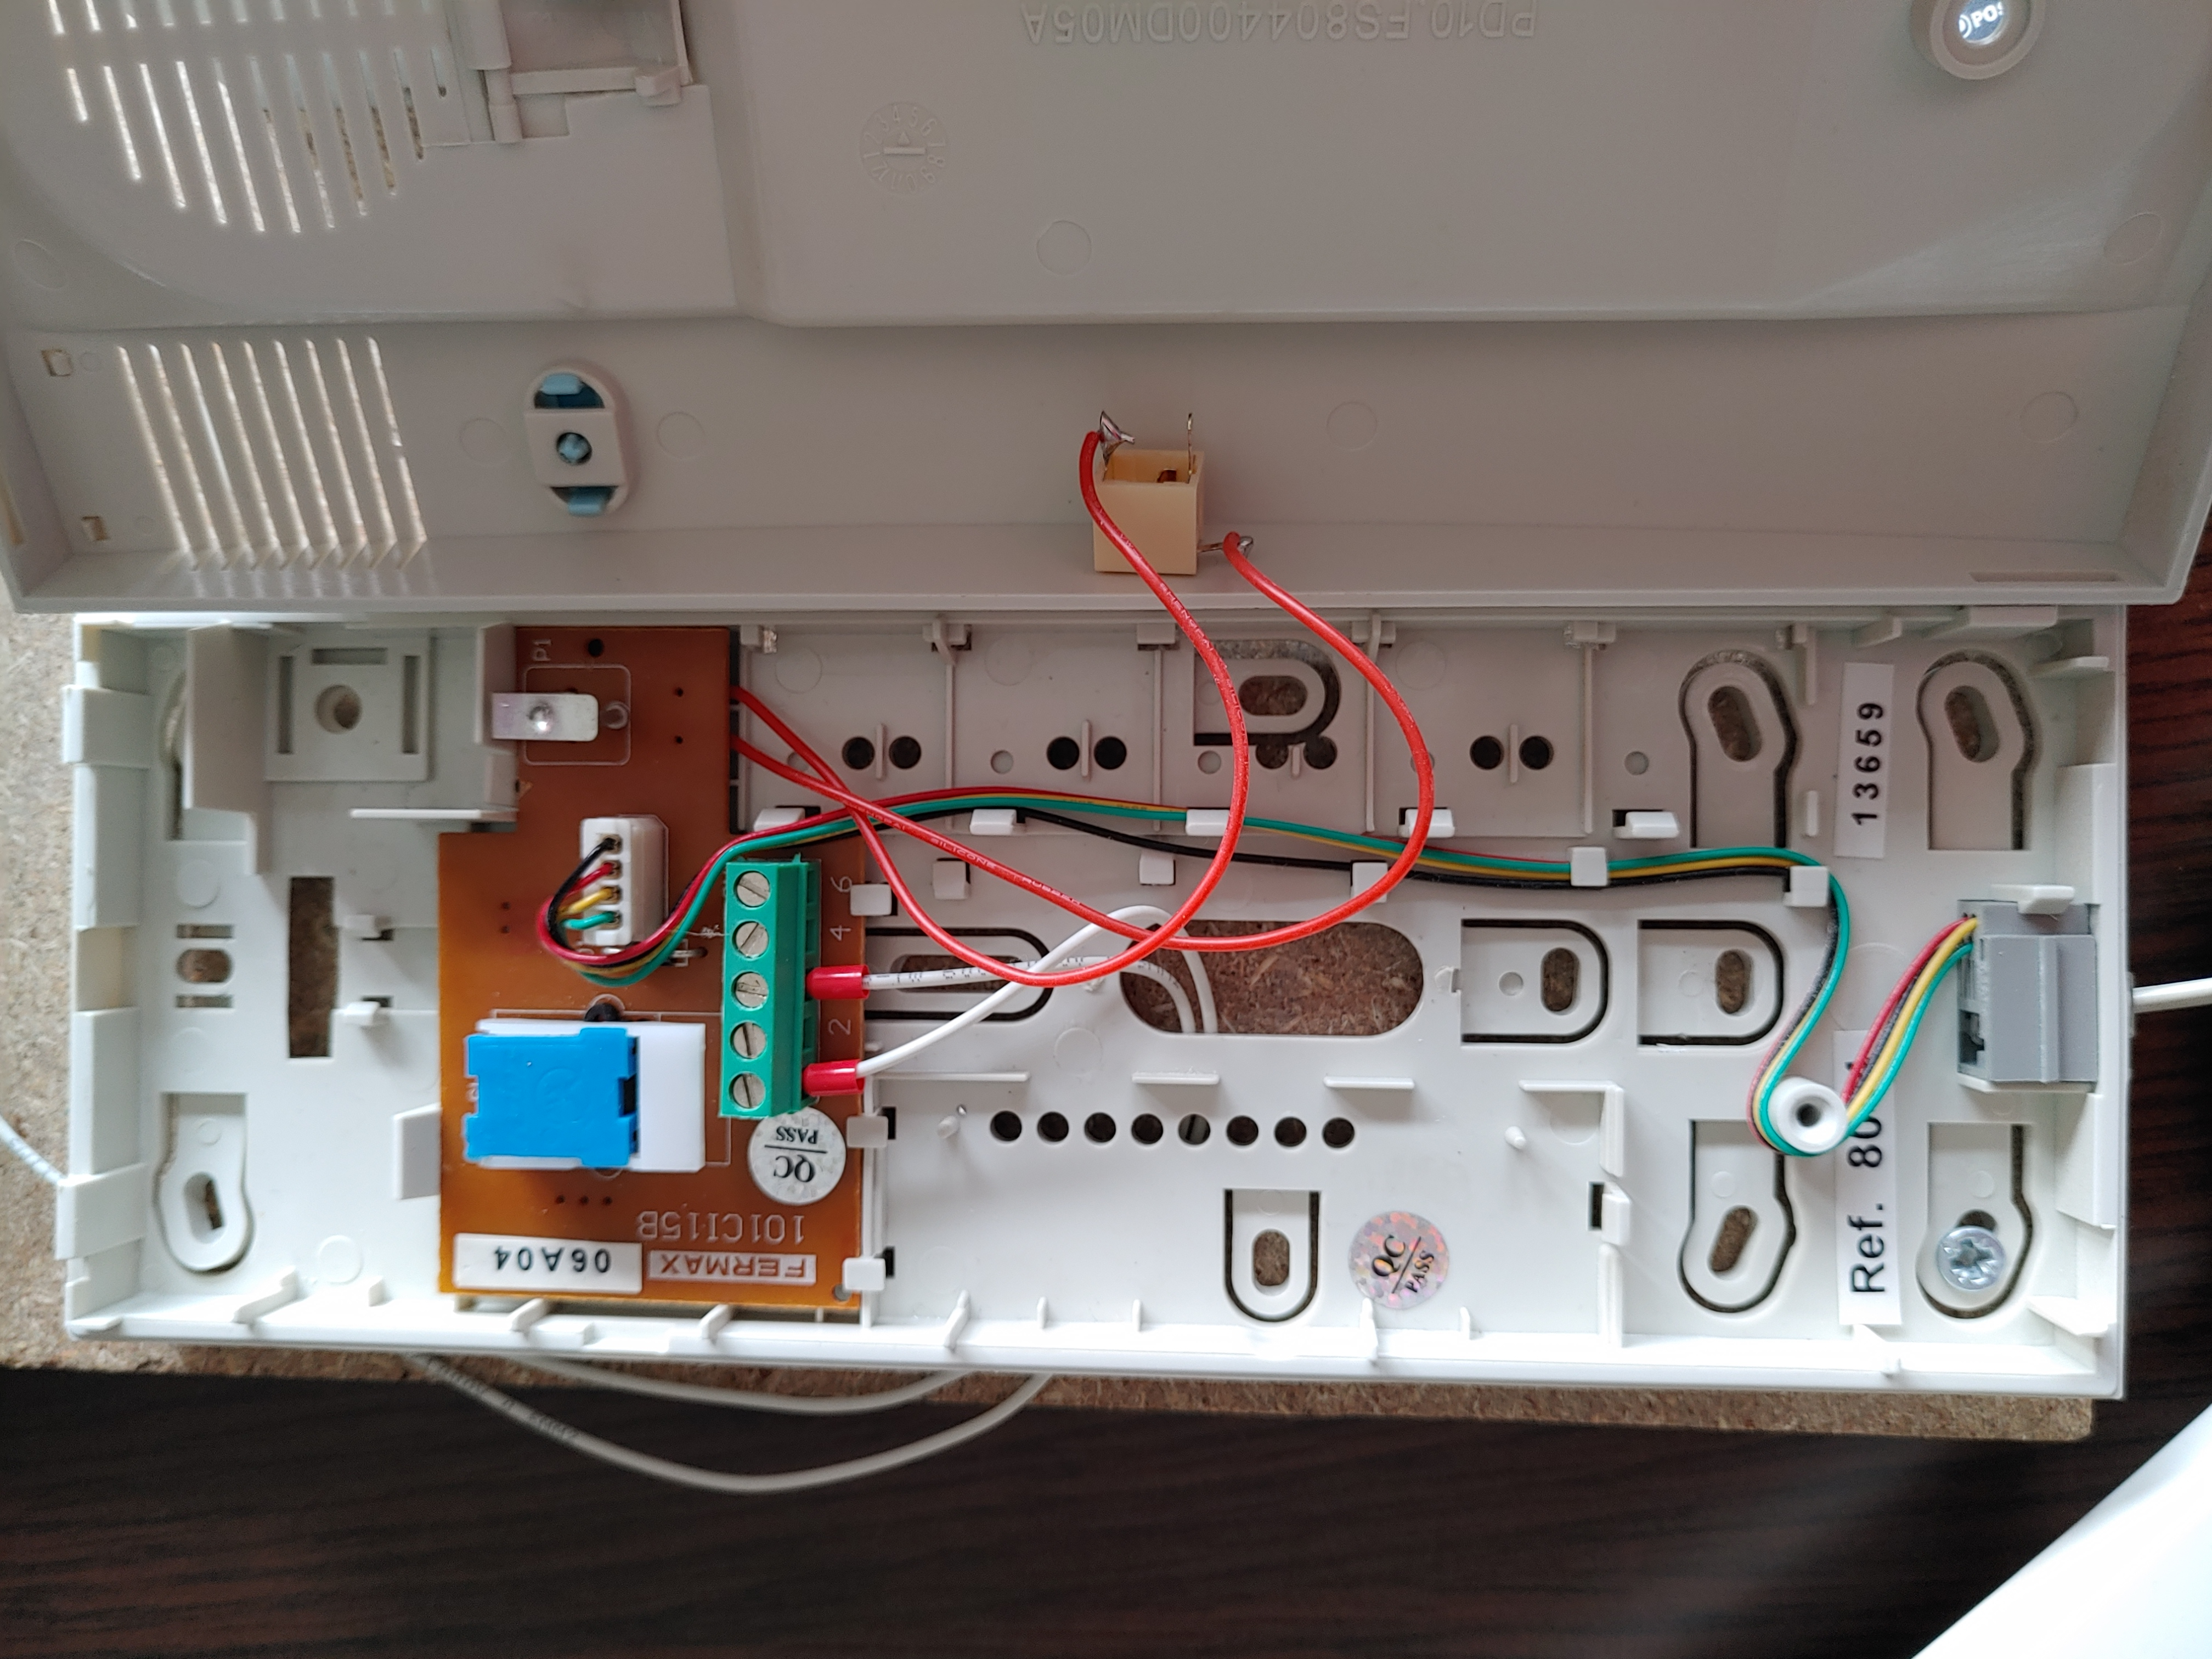
\includegraphics[scale = 0.1]{Interior_Portero_Automatico.jpg}
\caption{Conexiones en el interior del portero automático}
\label{fig:interior-portero-automatico}
\end{figure}

En las figura~\ref{fig:prototipo-completo} y ~\ref{fig:interior-portero-automatico} se puede observar el prototipo con todos los elementos que lo forman interconectados entre sí, tal como se definió en la fase de desarrollo. Tanto el portero automático, como la cerradura eléctrica y el transformador, han sido fijados por medio de tornillería a un tablón de madera que permite realizar, de forma segura y compacta, el transporte del prototipo.

Junto a estos elementos, puede observarse la interconexión de la Raspberry Pi Zero W con el conversor de nivel lógicos y el relé, que permiten el correcto funcionamiento de este prototipo.

La interconexión que adapta el sistema con el portero automático se ha hecho por medio de un conector tipo mini jack, con la intención de hacer que sea más intuitivo para el usuario final.

Queda expuesto por tanto, de forma gráfica, como los dos puntos principales que quedaron definidos para esta fase inicial han sido cumplidos de forma exitosa.

\section{Diseño de algoritmos y programación}
En el apartado de planificación del presente trabajo queda constancia de las diferentes materias que debían tenerse en cuenta en lo referente al diseño de algoritmos y programación.

\subsection{Programa capaz de activar la cerradura en los momentos precisos}

La primera característica que se implementa en el proyecto es la de hacer un programa capaz de activar una señal que permita realizar la apertura de la cerradura, ayudándose para ello del circuito construido previamente. Este programa debía poder estar controlado por un administrador que contara con la posibilidad de crear y anular reservas, realizar la apertura de la puerta y dejar las tareas de administración.

Una vez realizada la integración de los códigos implementados en la fase de desarrollo, y ejecutados por medio de la Raspberry Pi, se obtienen los resultados esperados, dando lugar a un panel de administración como el que se observa en la figura~\ref{fig:panel-de-administrador}.
\begin{figure}[tbp]
\centering
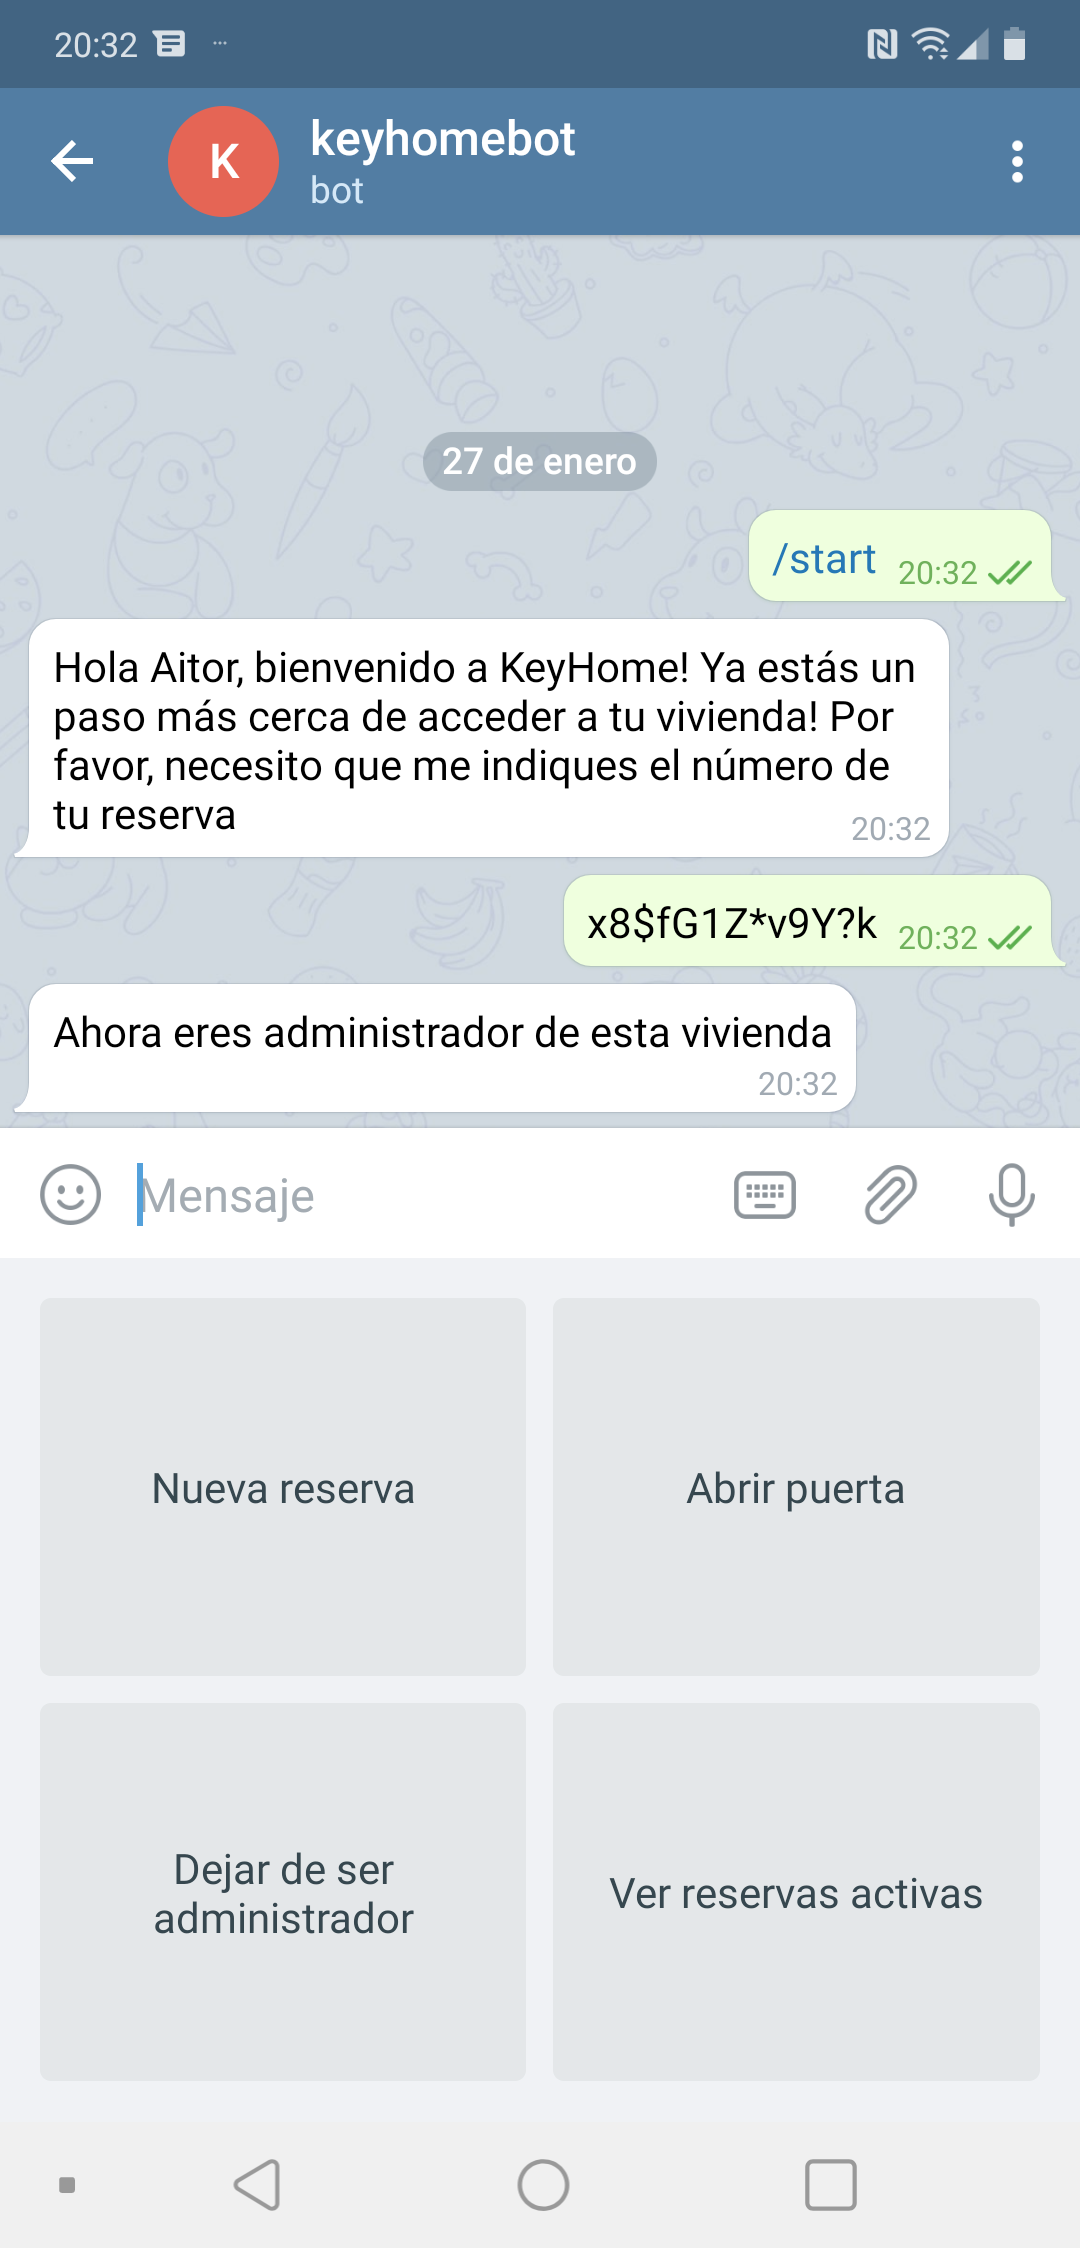
\includegraphics[scale = 0.15]{fig/Panel_de_administrador.png}
\caption{Panel de administrador}
\label{fig:panel-de-administrador}
\end{figure}

\subsubsection{Creación de nuevas reservas}

Entre las tareas de este apartado, destacan aquellas que tienen por objeto automatizar la entrada de nuevas reservas en el sistema. Sin embargo, por diferentes razones, es recomendable incluir la posibilidad al administrador de que él mismo pueda añadir estas reservas. Para ello, en la figura~\ref{fig:panel-de-administrador} se puede observar como se ha creado un apartado de crear reservas. Si hacemos uso de esta opción, el bot pedirá, en primer lugar, que se indique el número de reserva, tal como se puede observar en la figura~\ref{fig:introduccion-del-numero-de-reserva}. Este número de reserva será aquel con el que el huésped podrá acceder a la vivienda el día en que comience su estancia.
\begin{figure}[tbp]
\centering
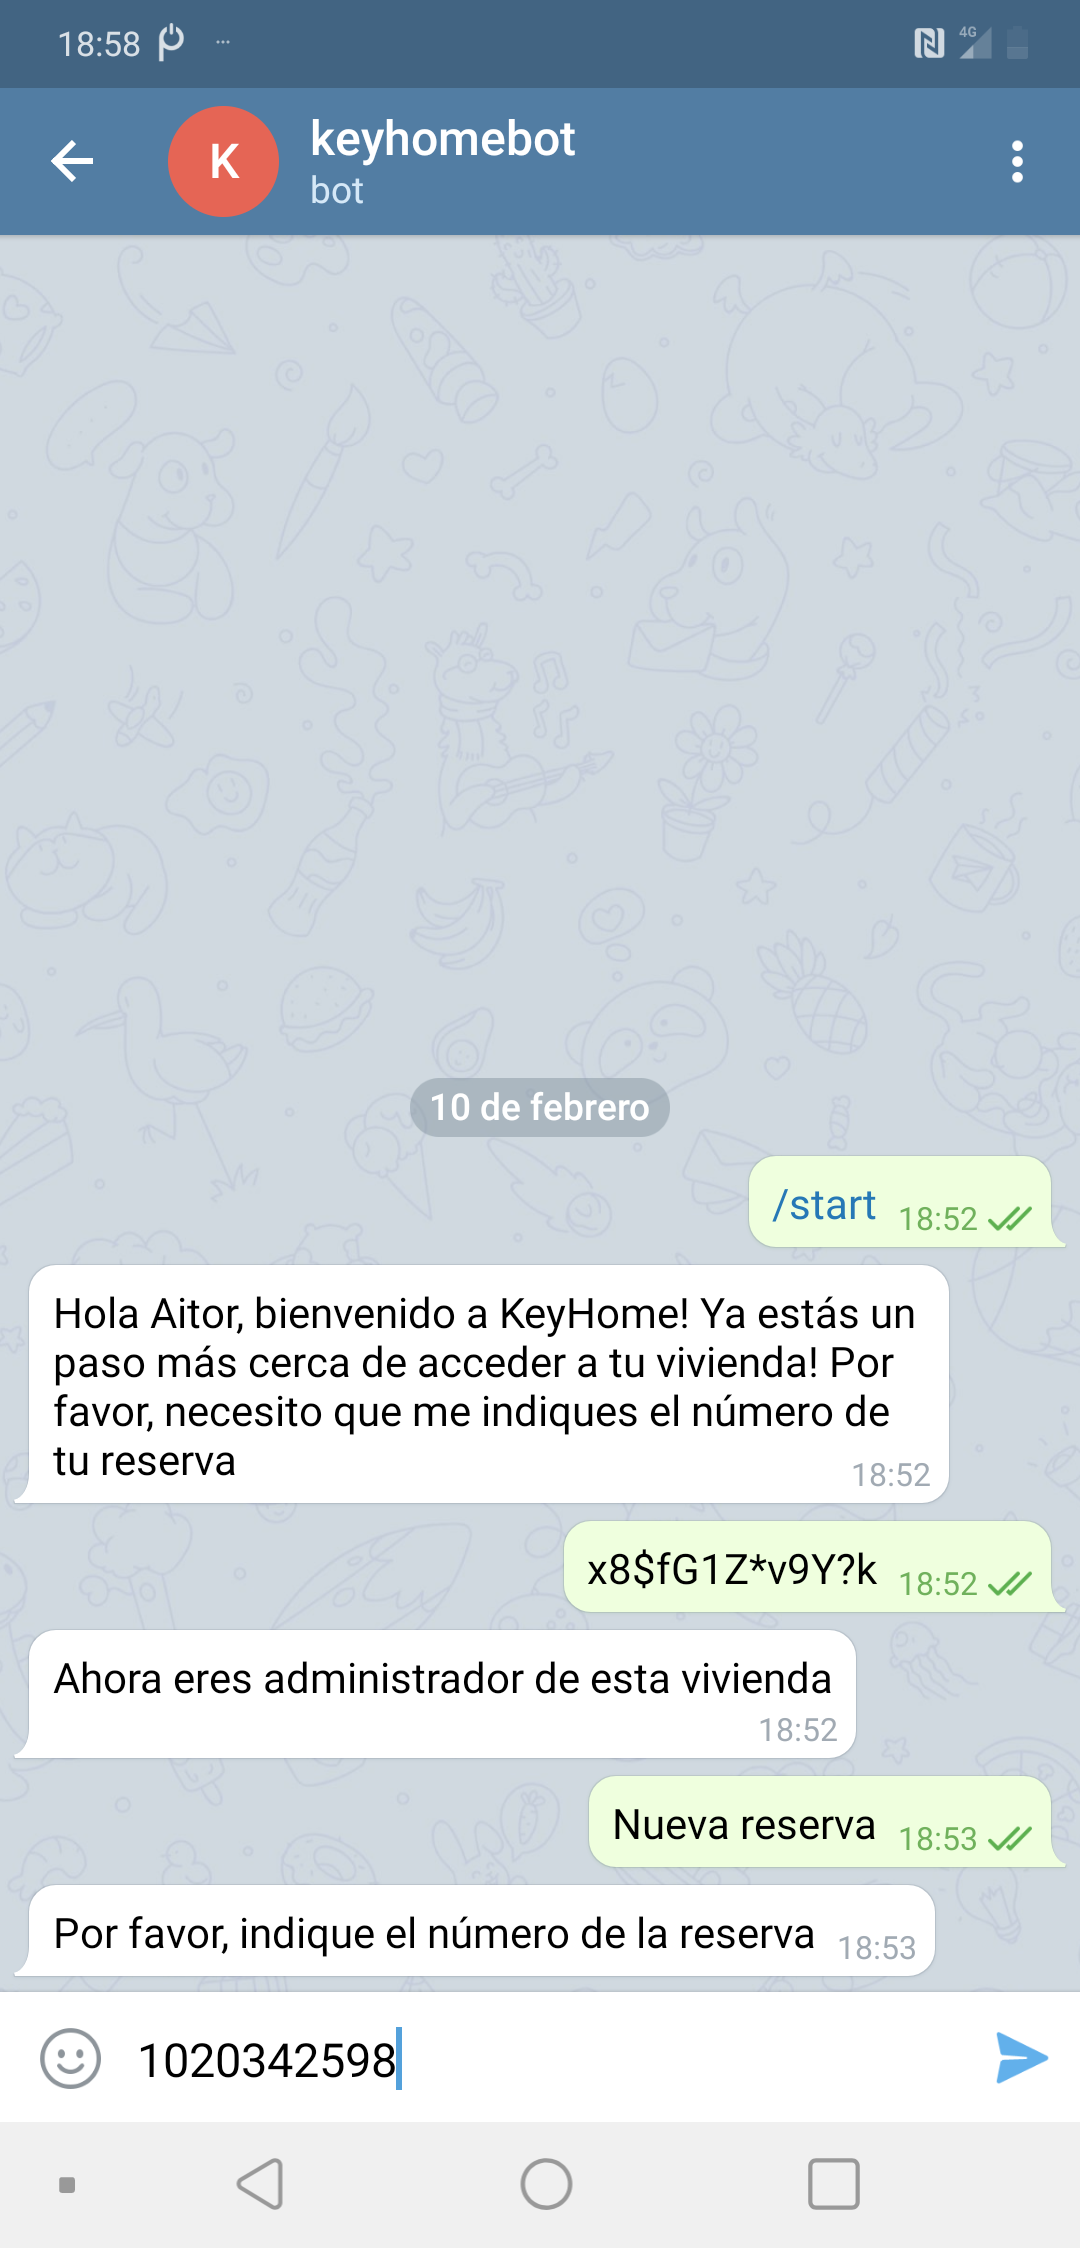
\includegraphics[scale = 0.15]{fig/Numero-de-reserva.png}
\caption{Introducción del número de reserva}
\label{fig:introduccion-del-numero-de-reserva}
\end{figure}

Una vez que el administrador introduzca el número de reserva, lo siguiente que le es exigido por parte del bot son las fechas de entrada y de salida del cliente, tal como puede observarse en la figura~\ref{fig:introduccion-de-las-fechas-de-reserva}, donde se establecen las fechas en las que el cliente podrá acceder a la vivienda.

\begin{figure}[tbp]
\centering
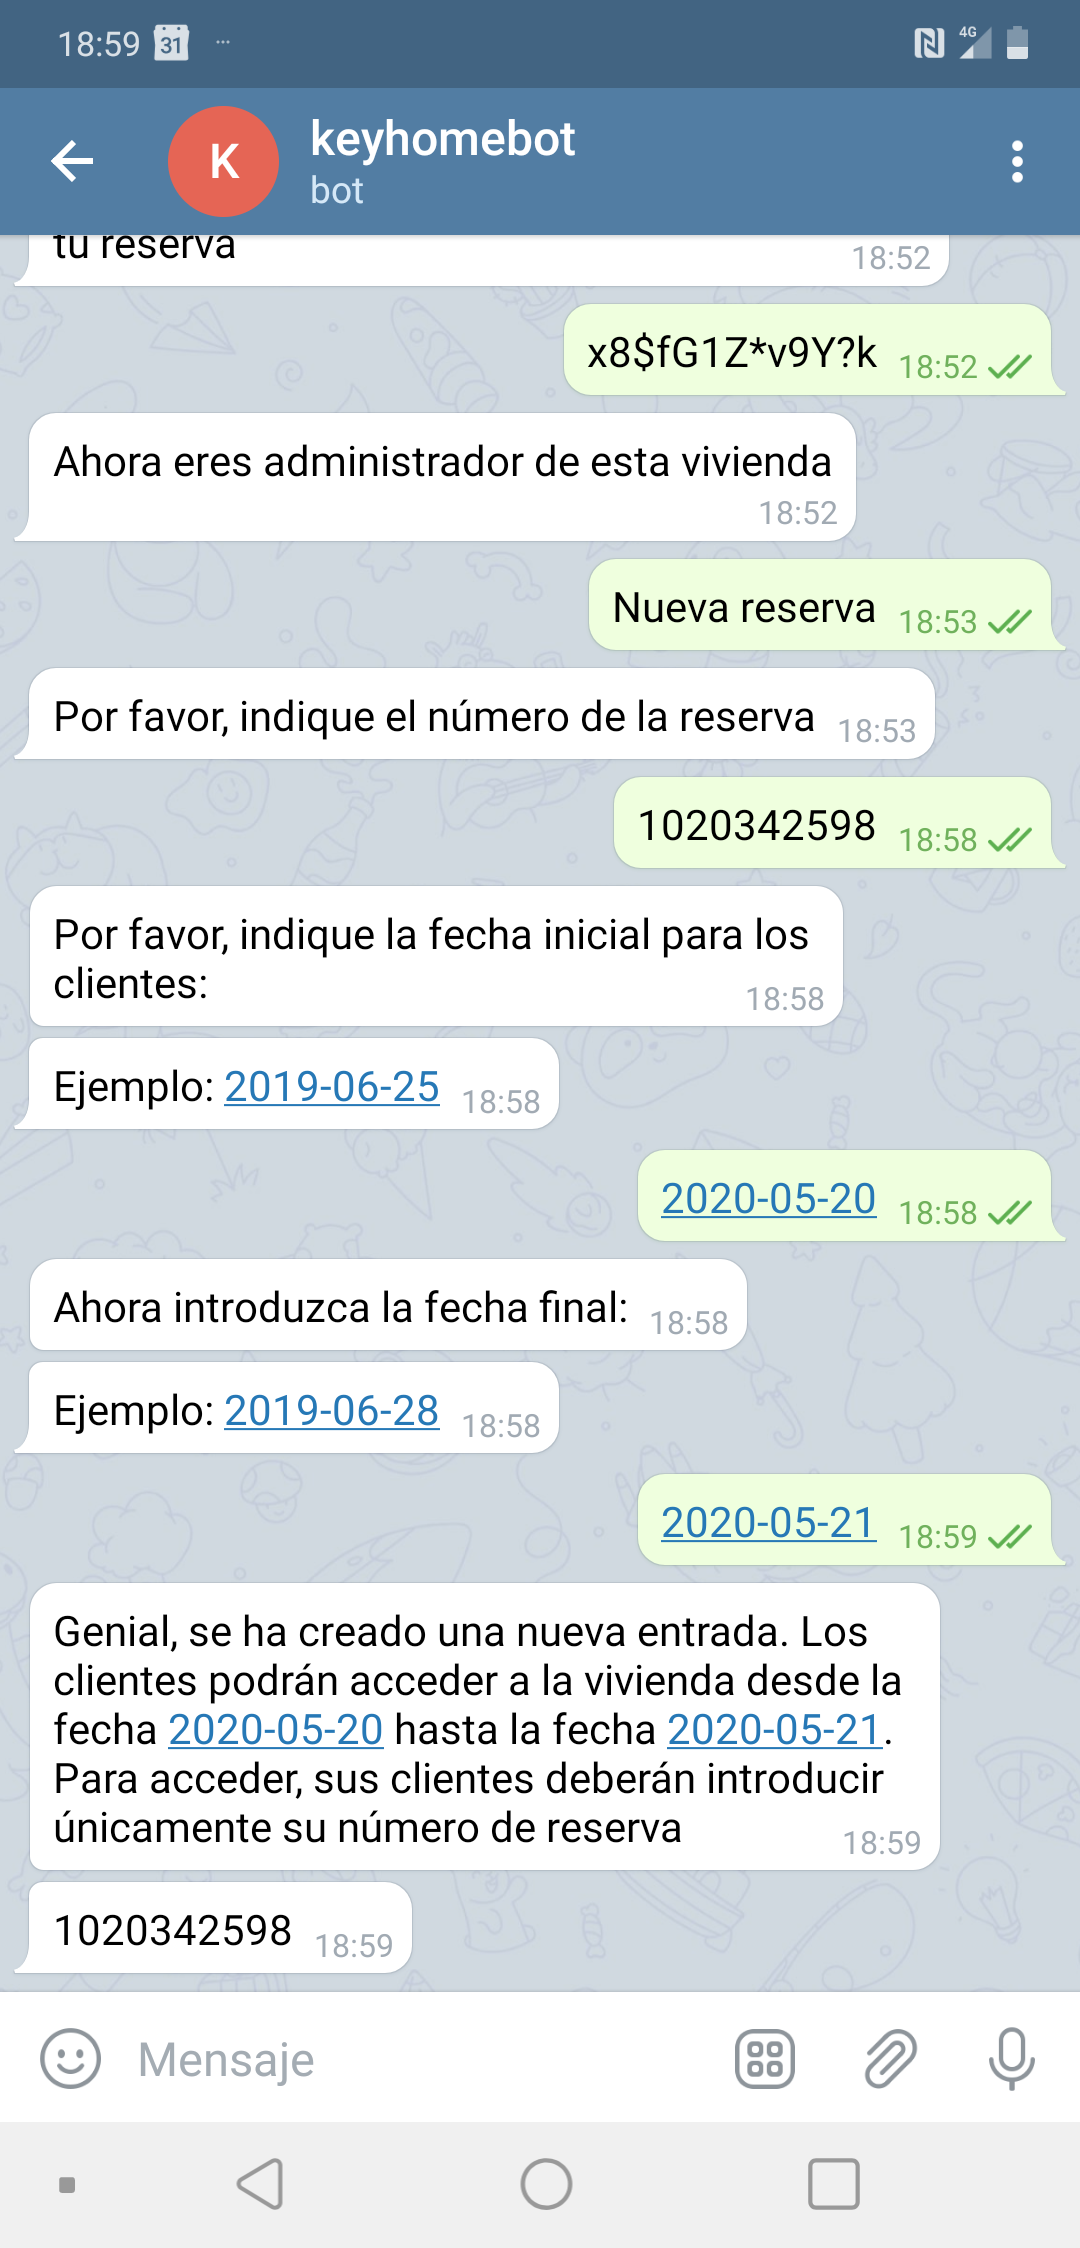
\includegraphics[scale = 0.15]{fig/Fechas-de-reserva.png}
\caption{Introducción de las fechas de reserva}
\label{fig:introduccion-de-las-fechas-de-reserva}
\end{figure}

\subsubsection{Apertura de la cerradura por parte del administrador}

La siguiente función que debe cumplirse, siguiendo la programación de las tareas, sería la de permitir que el administrador de la vivienda tuviese la posibilidad de abrir la puerta. Esta posibilidad queda habilitada en el programa central definido en el apartado de desarrollo de este documento, a través del cual se crea el resultado que se muestra en la figura~\ref{fig:apertura-de-puerta-por-parte-del-administrador}, donde un administrador activa la apertura de la cerradura desde su panel de control.

\begin{figure}[tbp]
\centering
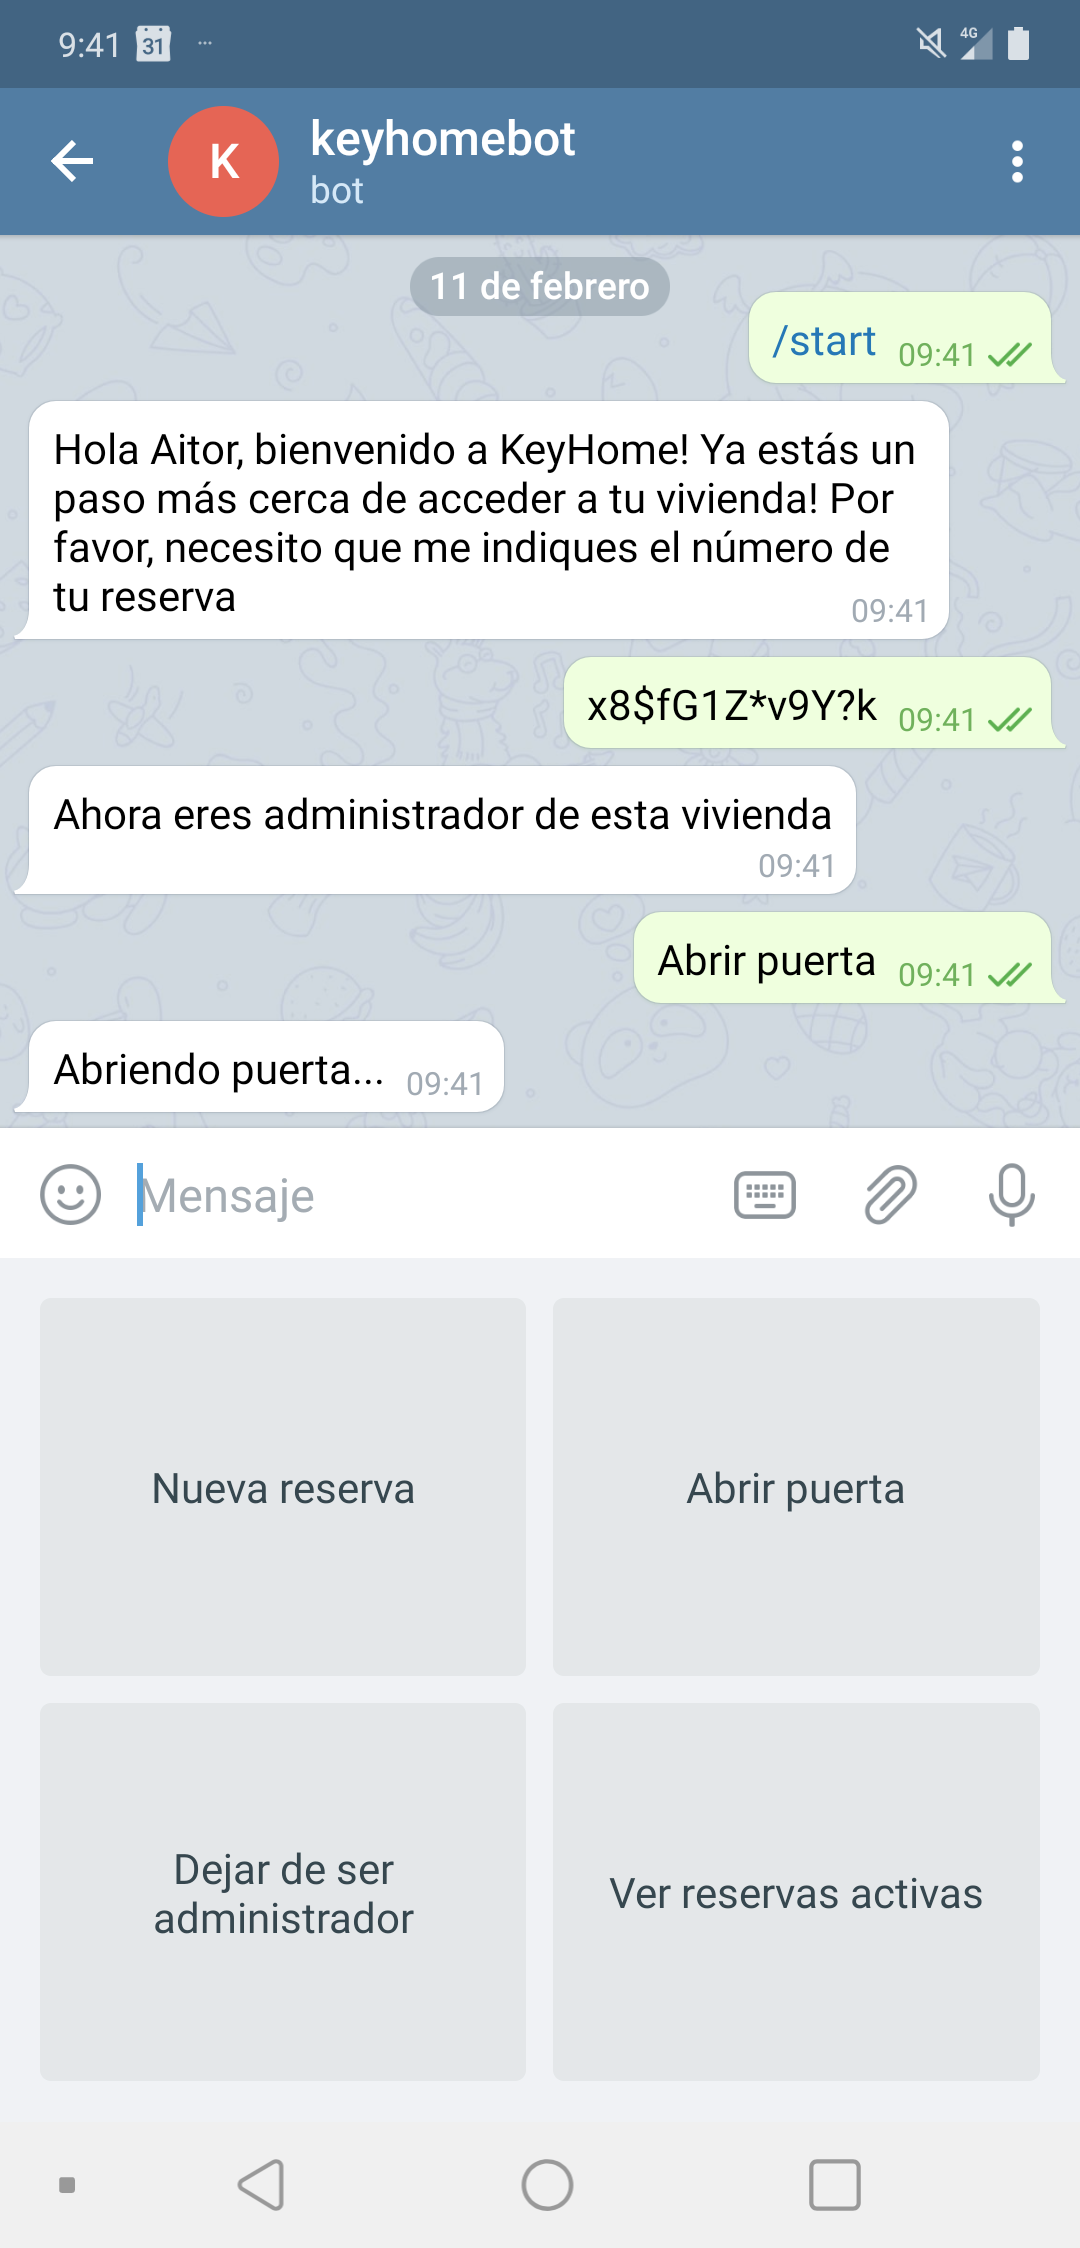
\includegraphics[scale=0.15]{fig/Apertura-de-puerta-administrador.png}
\caption{Apertura de puerta por parte del administrador}
\label{fig:apertura-de-puerta-por-parte-del-administrador}
\end{figure}

\subsubsection{Dejar permisos de administrador}

Por diferentes razones, se puede dar la situación de que una persona que ha sido administradora de la vivienda durante un tiempo, no deba continuar ejerciendo como tal. Para ello, se decidió habilitar esta aplicación con la posibilidad de dejar ese cargo, tal como puede observarse en la figura~\ref{fig:administrador-dejando-sus-permisos-de-administracion}, donde un administrador deja los permisos como administrador.

\begin{figure}[tbp]
\centering
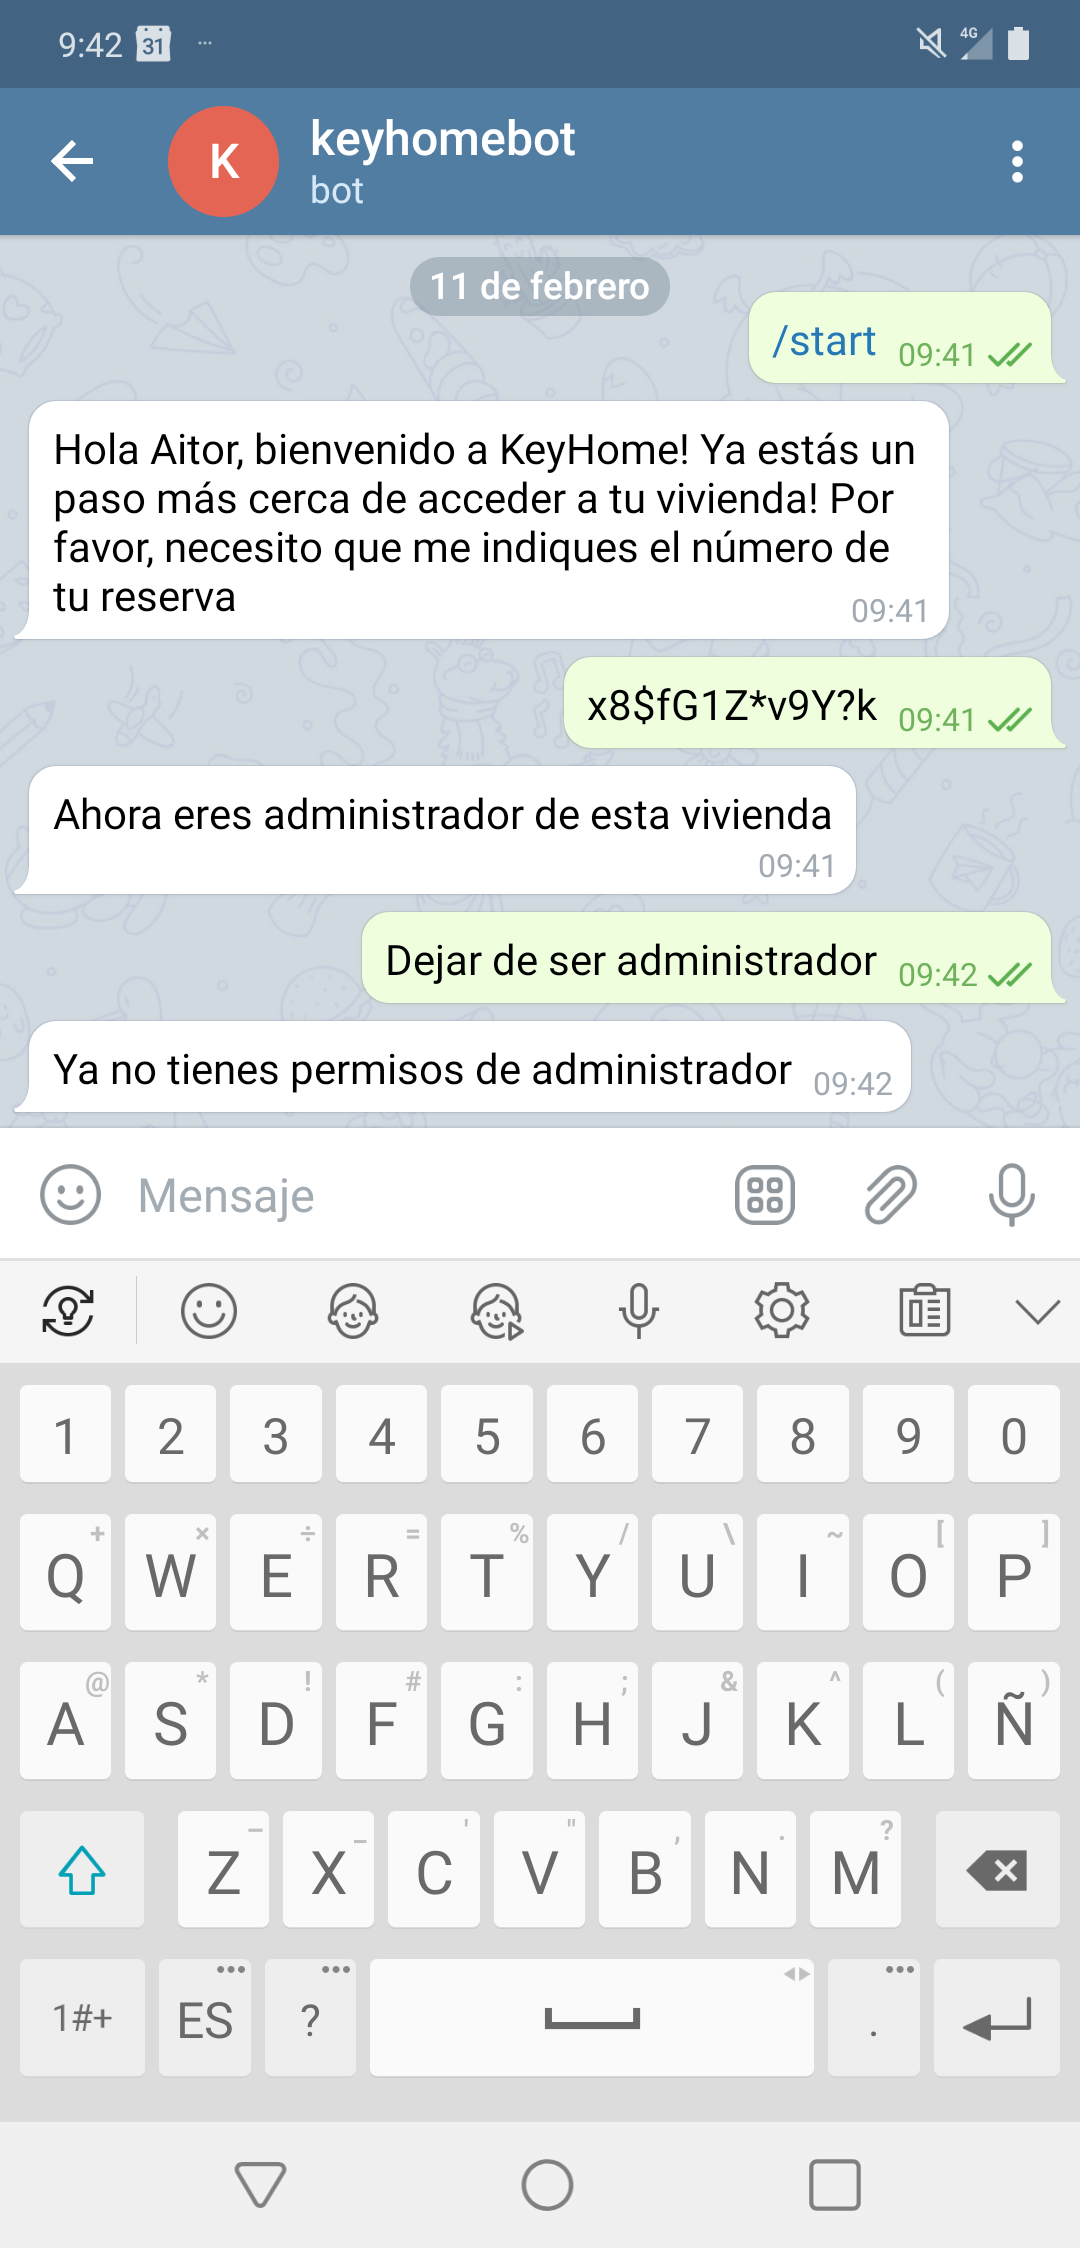
\includegraphics[scale=0.15]{fig/Dejar-de-ser-administrador.png}
\caption{Administrador dejando sus permisos de administración}
\label{fig:administrador-dejando-sus-permisos-de-administracion}
\end{figure}

\subsubsection{Consulta y modificación de reservas}

El último punto que se determinó añadir a los poderes de administrador, fue el de incluir la posibilidad de consultar las reservas, y además, poder anular aquellas que se considere. Es en la figura~\ref{fig:consulta-y-moficicacion-de-reservas}, donde se observa como el administrador de la vivienda consulta las diferentes fechas que hay disponibles, eliminando una de ellas a modo de ejemplo.

\begin{figure}[tbp]
\centering
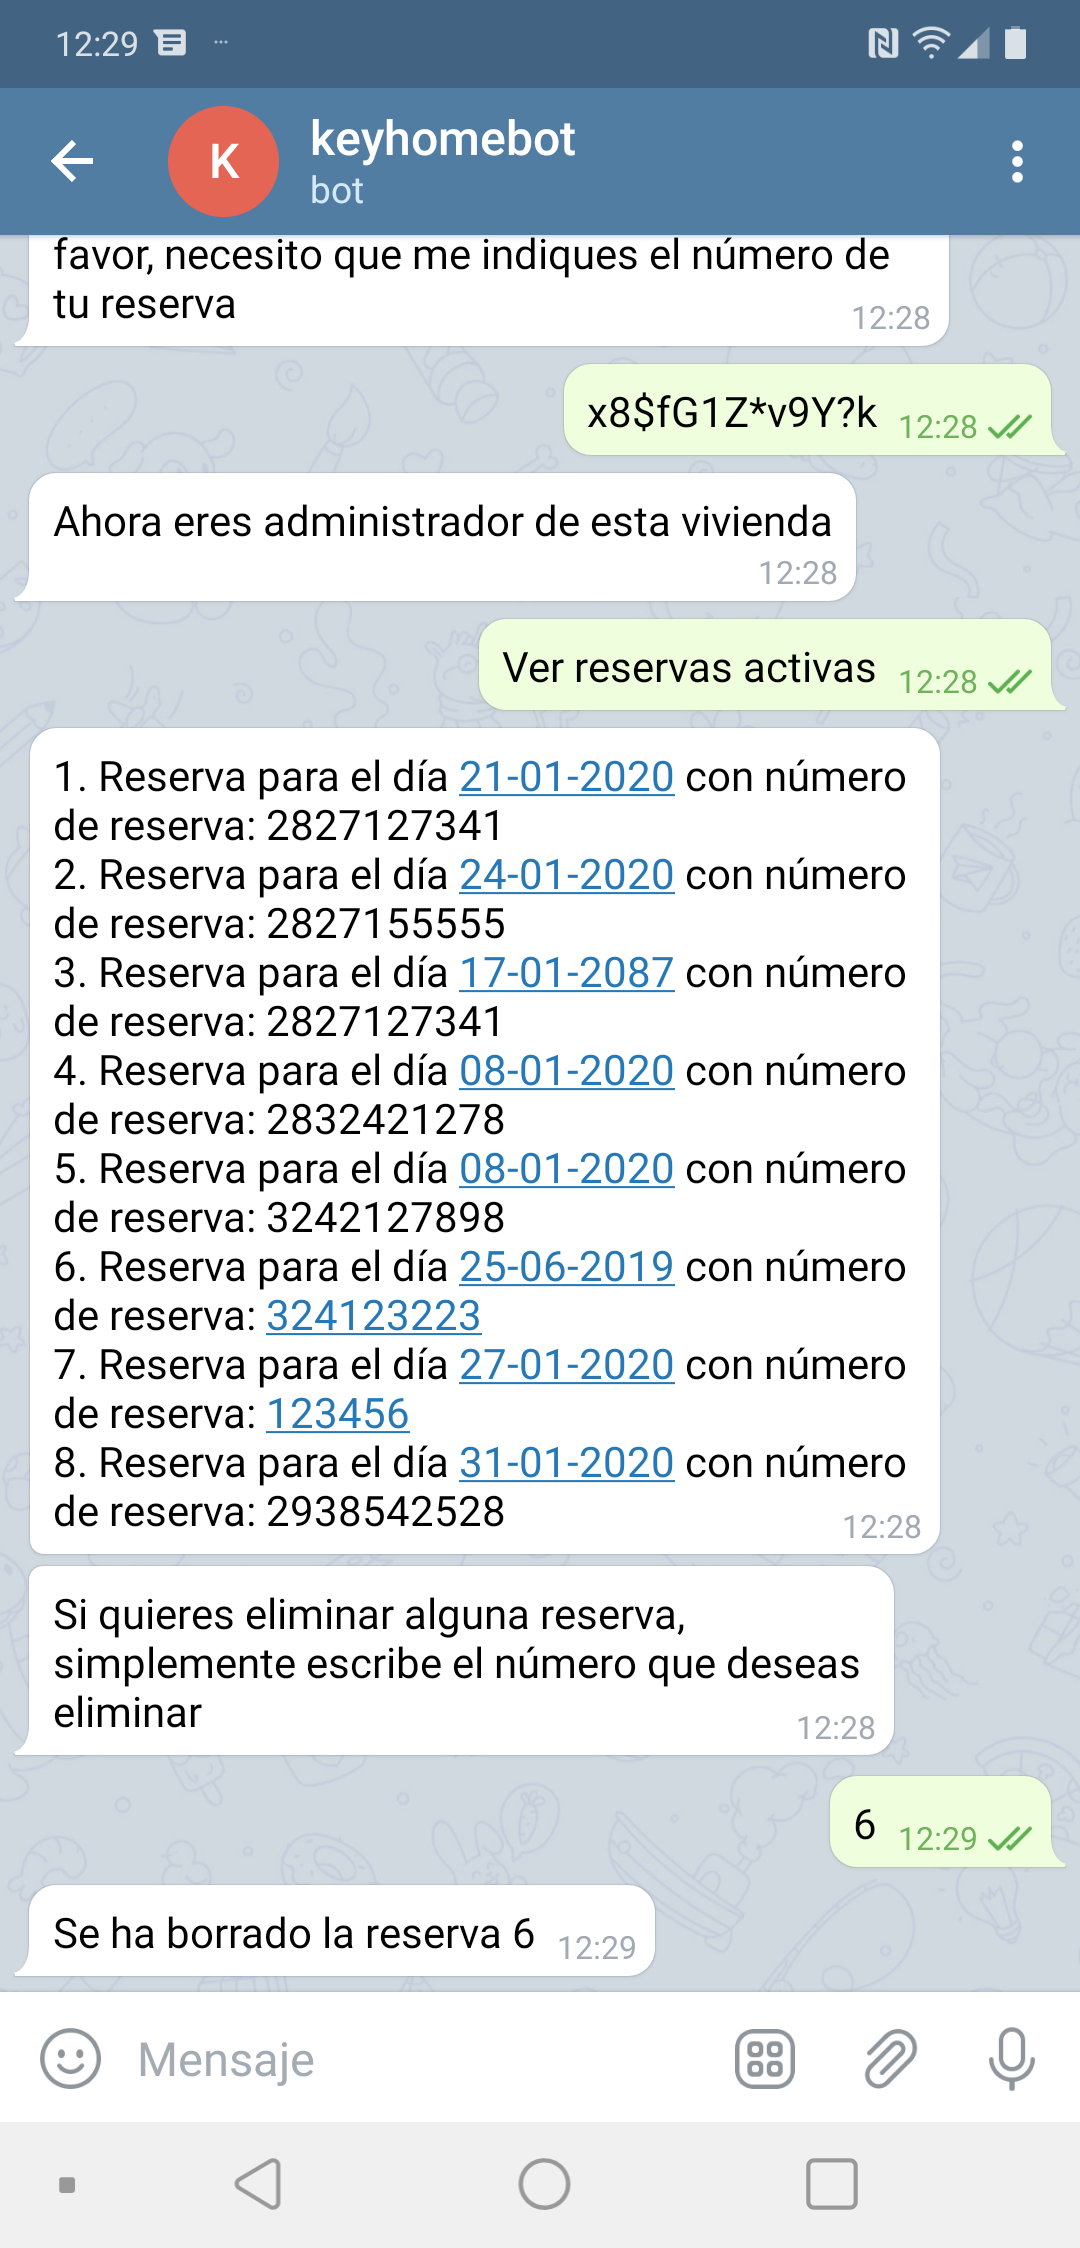
\includegraphics[scale=0.15]{fig/Consulta-y-modificacion-reservas.png}
\caption{Consulta y modificación de reservas}
\label{fig:consulta-y-moficicacion-de-reservas}
\end{figure}

A parte del administrador, la única figura que forma parte de este proyecto es la del usuario final o huésped de la vivienda, el cual debe tener a su disposición la posibilidad de abrir la puerta en el momento de su llegada. En la figura~\ref{fig:apertura-de-puerta-por-parte-del-huesped} puede observarse como este usuario final introduce su número de reserva, y al estar activo en ese momento, se le permite acceder a la vivienda realizando la apertura automática de la cerradura.

\begin{figure}[tbp]
\centering
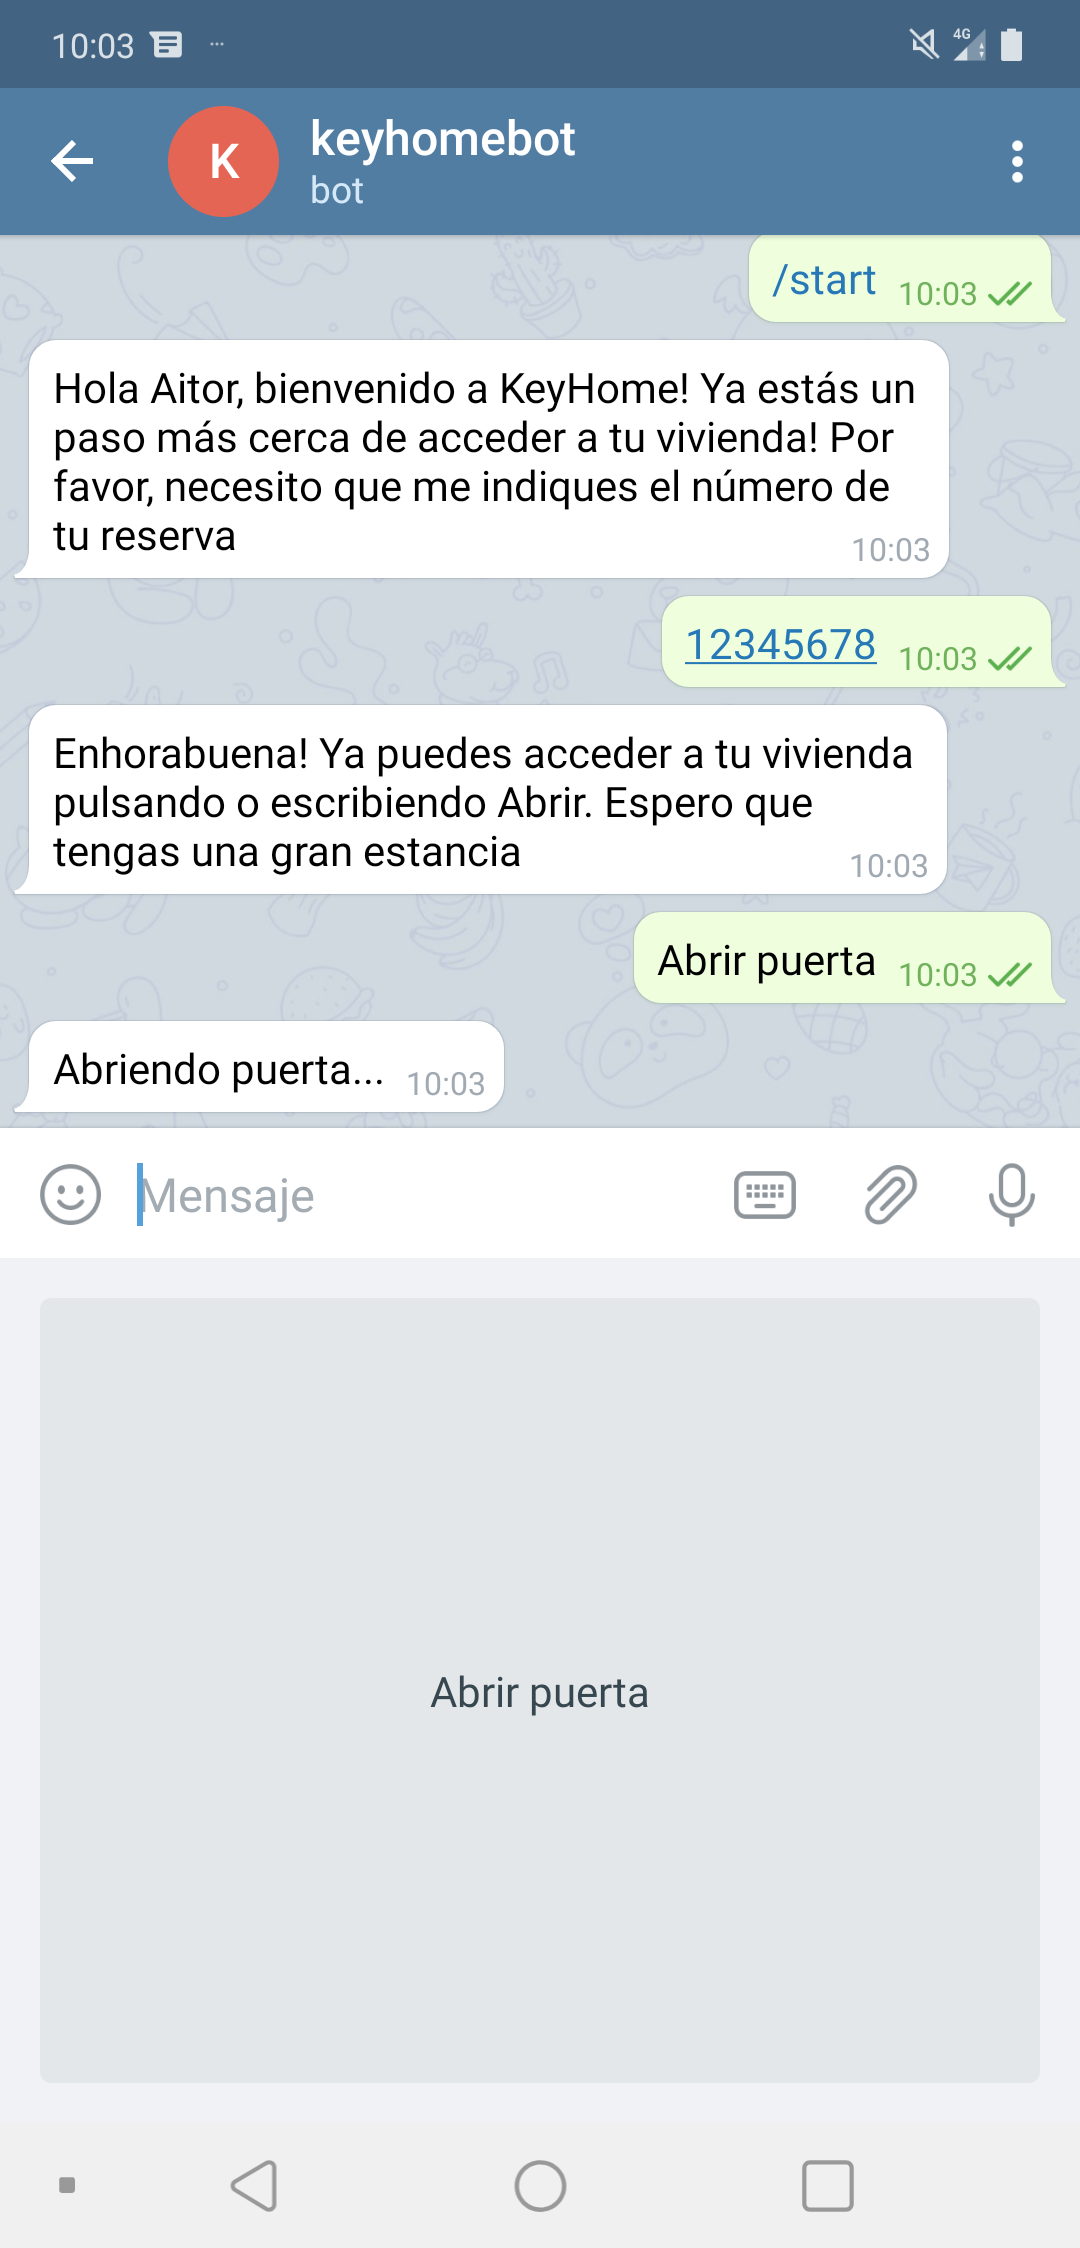
\includegraphics[scale=0.15]{fig/Apertura-de-puerta-por-parte-del-huesped.png}
\caption{Apertura de la cerradura por parte del huésped}
\label{fig:apertura-de-puerta-por-parte-del-huesped}
\end{figure}

\subsubsection{Automatización de la entrada y cancelación de reservas}

Existen muchas plataformas de alquiler vacacional. Para la elaboración de este sistema automático de recepción de reservas se ha hecho un programa, descrito en el apartado de desarrollo del presente documento, que automatiza las reservas de la plataforma Booking. Se ha tomado esta decisión, en base a dos razones principales:
\begin{enumerate}
\item Es la plataforma más utilizada en la actualidad.
\item Para la elaboración de este programa se ha podido utilizar el modelo de correo que envía Booking en la actualidad, con lo que la automatización descrita en este punto es completamente funcional.
\end{enumerate}

El resultado obtenido en este apartado ha sido el esperado, ya que ante una entrada de nueva reserva, notificada a la aplicación por medio de correo electrónico recibido de Booking, se ha conseguido incorporar dicha reserva en el historial de reservas que pueden ser consultados y modificados por el anfitrión. De igual manera, cuando Booking informa de una cancelación, por medio de un correo electrónico, este es recibido por el programa descrito en el apartado de desarrollo, el cual se encarga de eliminar dicha reserva del sistema incorporado en la Raspberry Pi, eliminando así toda posibilidad de acceso para el cliente que ha cancelado.

\subsection{Seguridad del dispositivo}
Al igual que en los puntos que preceden a este, la metodología de análisis de resultados consistirá en evaluar los frutos que han sido obtenidos del trabajo desempeñado en la fase de desarrollo.

El primer programa que se realizó consistía en un sistema de detección que avisara al propietario en caso de que alguien abriera la caja donde se encuentra el circuito.
El funcionamiento de este programa es correcto, actuando de manera que, en caso de que alguien abra la caja, el detector de distancia ofrecerá una medida mayor, y ante tal suceso, el programa enviará un correo electrónico como el que puede verse en la figura~\ref{fig:aviso-ante-posible-manipulacion}.

\begin{figure}[tbp]
\centering
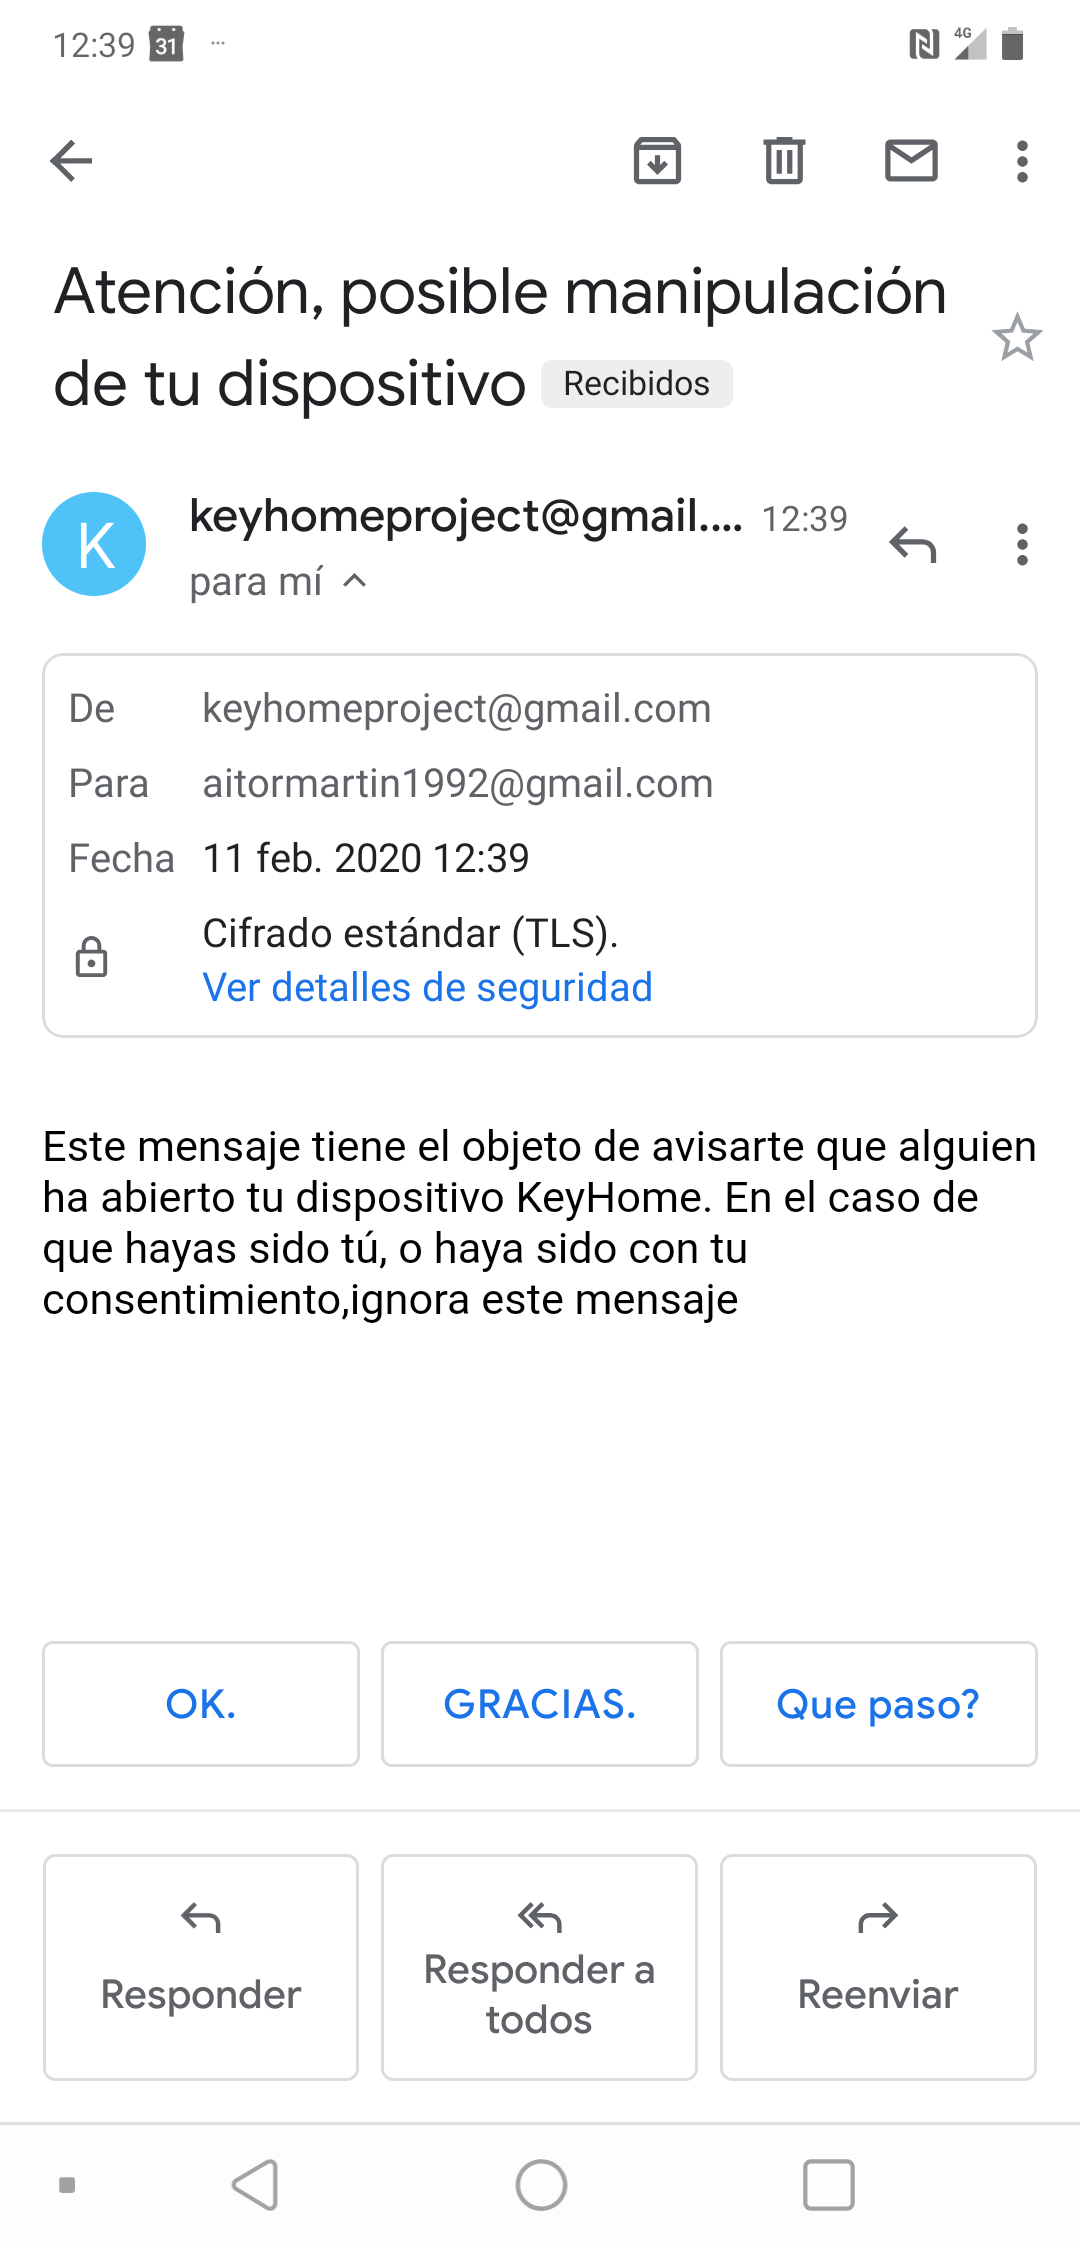
\includegraphics[scale=0.15]{fig/Aviso-ante-posible-manipulacion.png}
\caption{Aviso ante posible manipulación del dispositivo}
\label{fig:aviso-ante-posible-manipulacion}
\end{figure}

La desconexión, tanto a nivel eléctrico como de internet, del dispositivo, podría provocar múltiples situaciones negativas, como una posible manipulación o un cliente que no pudiera acceder a su vivienda. Para corregir esta situación, en la fase de desarrollo se decidió incluir un apartado en el que se avisara al propietario de forma remota. Para ello, se ha hecho uso de una plataforma llamada InitialState, que, tras la inclusión de ciertos scripts en la Raspberry Pi, recibe de forma continua señales de la ejecución del programa o programas que se deseen analizar. En la figura~\ref{fig:monitorizacion} puede observarse como, desde el ordenador, puede observarse de forma gráfica la frecuencia de trabajo de un programa en la Raspberry Pi.

\begin{figure}[tbp]
\centering
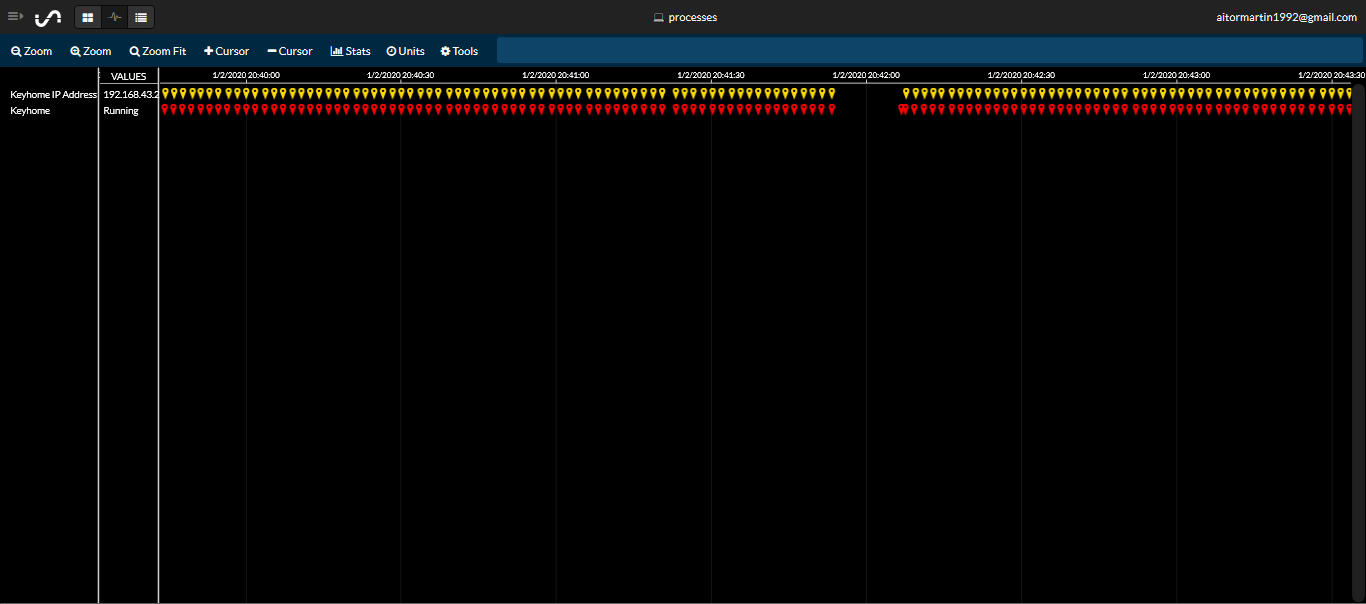
\includegraphics[scale=0.4]{fig/Monitorizacion.PNG}
\caption{Monitorización de la ejecución de un programa en la Raspberry Pi}
\label{fig:monitorizacion}
\end{figure}

En el caso de que se produzca una interrupción en el funcionamiento, el sistema de aviso alertará al propietario de la vivienda advirtiéndole de lo sucedido, tal como puede observarse en la figura~\ref{fig:aviso-ante-interrupcion-del-funcionamiento}. De esta manera, el anfitrión tendrá constancia de lo sucedido y podrá tomar las medidas que considere oportunas, como puede ser intercambiar la microSD de la Raspberry Pi para salvar posibles manipulaciones que pudieran haber ocurrido, o incluir por medio de su panel de control en Telegram las reservas que hubieran llegado en ese periodo de inactividad.

\begin{figure}[tbp]
\centering
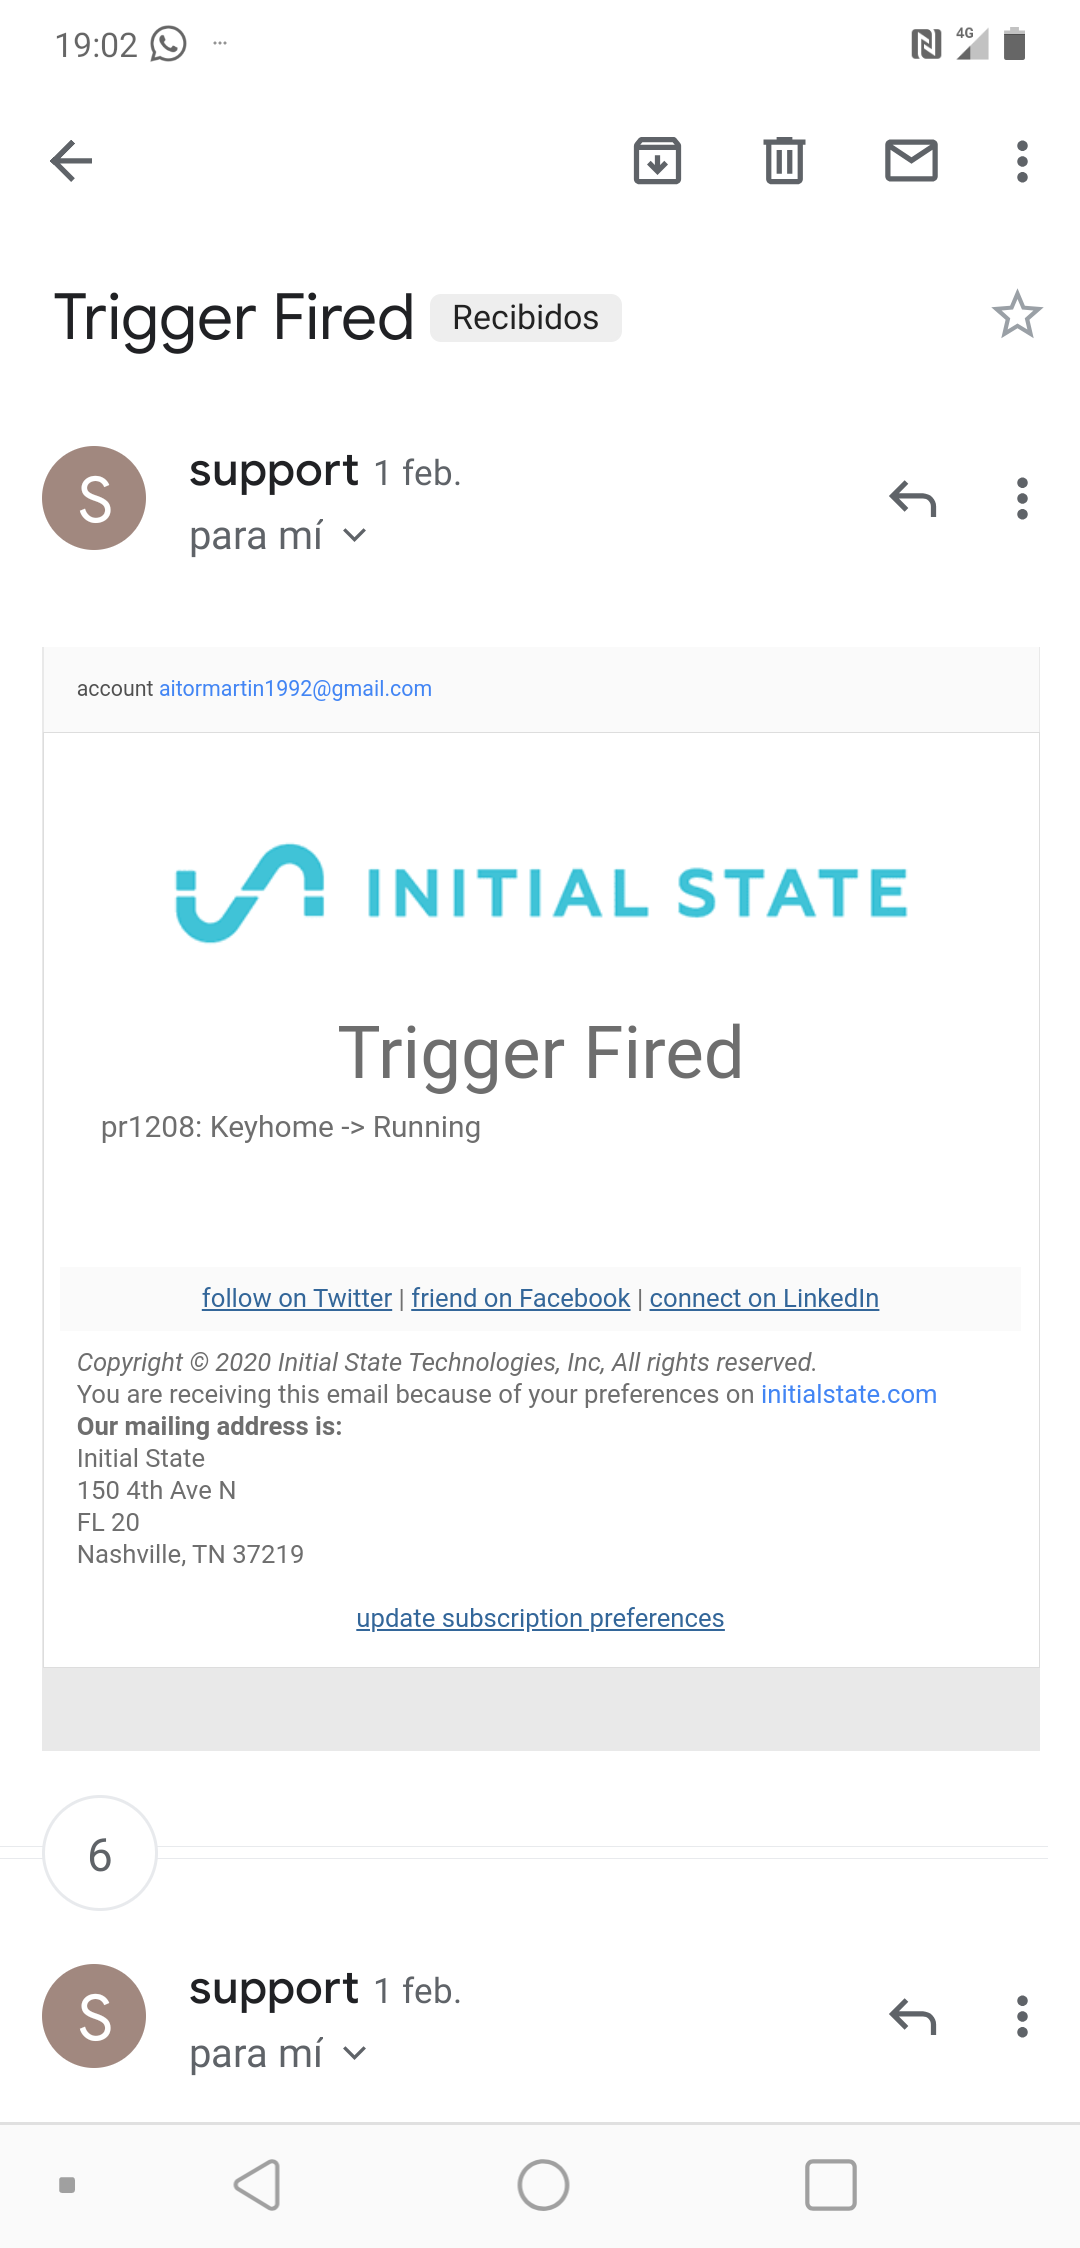
\includegraphics[scale=0.15]{fig/aviso-ante-interrupcion-del-funcionamiento.png}
\caption{Aviso ante una interrupción del funcionamiento}
\label{fig:aviso-ante-interrupcion-del-funcionamiento}
\end{figure}

\chapter{Discusión de resultados}
\label{ch:discusion-resultados}

Los resultados obtenidos a lo largo del desarrollo de este trabajo de fin de grado han sido en gran medida satisfactorios. El objetivo de automatizar por completo la reserva de un apartamento turístico ha sido llevado a cabo con éxito. Se presenta como resultado, por tanto, un producto funcional que ofrece un servicio adecuado y seguro para llevar a cabo la labor que es objeto de este proyecto.

No obstante, como todo avance tecnológico, la investigación y el desarrollo se han encontrado con aspectos positivos y también negativos, que vale la pena mencionar para poner en situación al lector y hacer que tenga una comprensión más profunda sobre el tema que se está tratando.

\section{Aspectos positivos}
\subsection{Instalación sencilla}
Uno de los aspectos positivos que vale la pena considerar es el hecho de que la instalación para el usuario final del dispositivo resultante de este proyecto tiene un carácter bastante sencillo. Únicamente deberá instalarse el aparato junto al portero automático conectado a un enchufe por medio de un cargador tipo USB micro B, disponible en multitud de comercios. El resto de la instalación consiste tan solo en conectar la hembra del conector mini jack en el telefonillo y poner cada uno de sus bornes en contacto con los puertos que permitan la apertura de la cerradura eléctrica desde el portero automático. Por ello, se obtiene un producto que puede instalarse en pocos minutos sin necesidad de conocimientos profundos en materia eléctrica o informática.
\subsection{Uso intuitivo}
El proyecto se ha desarrollado con éxito permitiendo tanto la gestión de la vivienda como el acceso a usuarios finales desde la aplicación de mensajería instantánea Telegram. El hecho de que sea la mensajería instantánea la que intermedie en todo momento hace que se presente un producto intuitivo y fácil de usar para multitud de usuarios que, en su vida diaria ya están acostumbrados a tratar con este tipo de aplicaciones.
\subsection{Producto seguro}
El resultado que se expone en este documento ha trabajado la seguridad en todos los aspectos posibles, desde su nivel más físico, impidiendo el acceso a la Raspberry Pi por medio de un diseño de impresión 3D protegido con candado, hasta sus niveles más sofisticados, avisando al administrador en caso de que se produzca una apertura o de que cualquier programa interrumpa su correcto funcionamiento. Este punto pone de manifiesto la importancia que se le da a la hora de proteger las residencias de aquellas personas que puedan interesarse por el producto.
\section{Aspectos negativos}
\subsection{Un mercado hermético}
Cabe destacar, sin embargo, que las posibilidades de aplicaciones que ampliarían la escalabilidad de este proyecto se ven comprometidas por la propia forma en que se estructura el mercado de las vivienda de uso turístico. En España, este negocio multimillonario es controlado y dirigido principalmente por 2 empresas (Booking y Airbnb) las cuales son bastante restrictivas a la hora de permitir trabajar con sus APIs.

Tan solo unas pocas empresas, que actúan como channel managers, tienen la posibilidad de trabajar con estos gigantes haciendo aplicaciones que actualicen los precios, gestionen las reservas, automaticen los registros de huéspedes para la policía, y otras muchas actividades que resultan de gran utilidad para los anfitriones. 

Este hecho provoca que la manera de trabajar para coger las reservas haya consistido, tal como se explica en el apartado de desarrollo del presente trabajo de fin de grado, en extraer la información necesaria de los correos electrónicos que notifican la información a los anfitriones. Este método, aunque se ha podido comprobar en este trabajo que funciona de manera correcta, no es la forma más eficiente de hacerlo, ya que podrían surgir problemas como el hecho de que las empresas de alquiler vacacional oculten información como las fechas de reserva o el número de reserva en los correos electrónicos, permitiendo tan solo acceder a los mismos desde el panel de administración de cada plataforma.

\subsection{Adaptación con cerraduras electromecánicas}
Una característica adicional que, por razones principalmente de coste, habría sido interesante llevar a cabo, sería la adaptación del sistema desarrollado con cerraduras inteligentes motorizadas. Activar la apertura con este tipo de cerraduras permitiría que no solo se emplearan cerraduras eléctricas en las viviendas donde se desee adaptar este sistema, si no que podría adaptarse a todo tipo de puertas y cerraduras, ofreciendo de esa manera, mayor seguridad ante robos o posibles allanamientos al usar infraestructuras más seguras.



\chapter{Conclusiones}
\label{ch:conclusiones}

Este trabajo de fin de grado ha concluido con éxito todos los objetivos propuestos en su apartado correspondiente. A nivel físico, se ha creado un circuito electrónico básico que, con la incorporación del software desarrollado, es capaz de cumplir con su cometido realizando la apertura de la cerradura eléctrica en los momentos que han sido planteados.

Adicionalmente, se han desempeñado exitosamente todas las tareas de desarrollo de software que se habían propuesto, tanto a nivel de funcionalidad, permitiendo la gestión integral de la vivienda y el acceso de los huéspedes, como a nivel de seguridad, teniendo en cuenta todos los posibles peligros que se consideraron en el análisis de este proyecto.

Como conclusión, se expone de este trabajo un proyecto completamente funcional que resuelve las tareas descritas y ofrece un servicio de utilidad a los posibles anfitriones que deseen hacer uso del mismo.

No obstante, este trabajo también cuenta con mejoras que no han sido tratadas, por cuestiones de tiempo y económicas, como son la implantación de este sistema en cerraduras inteligentes motorizadas o la integración de servicios de cálculo de precios, unificación de calendarios y otros servicios que pudieran hacer todavía más integral y útil este proyecto. Estas funcionalidades podrían ser tenidas en cuenta en una posible línea de investigación futura, que se apoye sobre el trabajo de este documento y la tecnología del momento.

Otros aspectos que serían relevantes para la evolución de este sistema a la hora de llevarlo a la realidad, sería la respuesta del propio público a la hora de utilizar estos sistemas automatizados. Todas las aplicaciones tecnológicas tienden a evolucionar con diferentes versiones, adaptándose a las necesidades del mercado según se van conociendo. En este caso no sería distinto, y la única forma de ver las mejoras que se deberían incluir, y los aspectos que se deberían considerar, sería probándolo directamente con clientes reales, que ayudarían a mejorar significativamente el valor de este producto.
